% ------------------------------------------------------------------------------
% Universidade Federal de Alagoas - UFAL
%
% Artigo científico (trabalho acadêmico) em conformidade com as normas da ABNT
% Tema: Avaliação observacional do Programa Pé-de-Meia (painel das 27 UFs)
%
% Modelo base: https://github.com/marceloqao/latex-UFAL
% (Marcelo Queiroz de A. Oliveira, com base no trabalho de Cristiano Nunes e
% Henrique Borges)
%
% COMPILAÇÃO (pdfLaTeX + BibTeX):
%   pdflatex meu-trabalho
%   bibtex   meu-trabalho
%   pdflatex meu-trabalho
%   pdflatex meu-trabalho
% ou simplesmente:  latexmk -pdf meu-trabalho.tex
% No Overleaf: Menu > Compiler = pdfLaTeX; Main document = meu-trabalho.tex
% ------------------------------------------------------------------------------

% Utiliza um modelo para impressão apenas no anverso
\documentclass[oneside]{ufal}

% ------------------------------------------------------------------------------
% Pacotes utilizados
% ------------------------------------------------------------------------------
\usepackage[utf8]{inputenc}         % Codificação do documento
\usepackage[T1]{fontenc}            % Seleção de código de fonte
\usepackage{booktabs}               % Réguas horizontais em tabelas
\usepackage{color, colortbl}        % Controle de cores
\usepackage{graphicx}               % Inclusão de gráficos
\usepackage{indentfirst}            % Recua o primeiro parágrafo de cada seção
%\usepackage[expansion=false]{microtype} % Opcional: comentado para acelerar a compilação no Overleaf
\usepackage{multirow, makecell}     % Tabelas com múltiplas linhas e colunas
\usepackage{verbatim}               % Exibe texto tal como escrito no documento
\usepackage{icomma}                 % Utiliza vírgulas em expressões matemáticas
\usepackage{amsmath}                % Funções matemáticas
\usepackage{amssymb}                % Símbolos matemáticos adicionais
\usepackage{newtxtext,newtxmath}    % Utiliza a fonte 'Times New Roman' (clone)
\usepackage{array}                  % Extensões de colunas em tabelas
\usepackage{tabularx}               % Tabelas com largura fixa
\usepackage{longtable}              % Tabelas que atravessam páginas
\usepackage{pdflscape}              % Páginas em paisagem (tabelas largas)
\usepackage{tikz}                   % Diagramas (fluxo do pipeline)
\usetikzlibrary{positioning, arrows.meta, calc, babel}

% Compatibilidade com URLs geradas pelo abntex2cite no .bbl
\AtBeginDocument{\def\htmladdnormallink#1#2{\href{#2}{#1}}}

% ------------------------------------------------------------------------------
% Configurações gerais
% ------------------------------------------------------------------------------

% Define o tamanho do recuo do parágrafo
\setlength{\parindent}{1.25cm}

% Define o espaçamento entre um parágrafo e outro
\setlength{\parskip}{0.0cm}

% Define a cor utilizada nos links do PDF
\definecolor{blue_link}{RGB}{0,80,128}

% Define as palavras-chave nos metadados do PDF
\hypersetup{pdfkeywords={%
    Pé-de-Meia, Diferenças em Diferenças, Abandono escolar, IDEB, Ensino Médio,
    Ciência de Dados.
}}

% Coluna centralizada com largura fixa (tabelas)
\newcolumntype{C}[1]{>{\centering\arraybackslash}p{#1}}
\newcolumntype{Y}{>{\centering\arraybackslash}X}

% Comando para nomes de arquivos, variáveis e colunas de dados
\newcommand{\arquivo}[1]{\texttt{\detokenize{#1}}}

% Define a hifenização de palavras que não estão no dicionário
\hyphenation{%
    Pé-de-Mei-a
    Cad-Ú-ni-co
    he-te-ro-ce-das-ti-ci-da-de
}

% ------------------------------------------------------------------------------
% Inclui os arquivos do trabalho acadêmico
% ------------------------------------------------------------------------------

% Inclui o arquivo que contém os dados do trabalho acadêmico
% ------------------------------------------------------------------------------
% Dados do trabalho acadêmico
% >>> ATENÇÃO: revise os campos marcados com [PREENCHER] antes de publicar <<<
% ------------------------------------------------------------------------------

\titulo{Avaliação observacional do Programa Pé-de-Meia}
\subtitulo{evidências de um painel das 27 Unidades da Federação (2019--2025) por Diferenças em Diferenças}
\autor{[Bruno Martins Gomes,
Samara Alves Pereira]}
\local{Penedo}
\data{Novembro de 2026} % Normalmente se usa apenas mês e ano

% ------------------------------------------------------------------------------
% Natureza do trabalho acadêmico
% ------------------------------------------------------------------------------

\projeto{Artigo científico}

% ------------------------------------------------------------------------------
% Título acadêmico (não se aplica a trabalho de disciplina; mantido vazio)
% ------------------------------------------------------------------------------

\tituloAcademico{}

% ------------------------------------------------------------------------------
% Dados da instituição
% ------------------------------------------------------------------------------

\instituicao{Universidade Federal de Alagoas}
\programa{[PREENCHER: Instituto/Curso] -- Disciplina de Ciência de Dados}

% ------------------------------------------------------------------------------
% Área de concentração e linha de pesquisa (vazios em trabalhos de graduação)
% ------------------------------------------------------------------------------

\areaconcentracao{}
\linhapesquisa{}

% ------------------------------------------------------------------------------
% Logomarca
% ------------------------------------------------------------------------------

\logoinstituicao{4cm}{figuras/logo_ufal_pb}

% ------------------------------------------------------------------------------
% Docente responsável pela disciplina
% ------------------------------------------------------------------------------

\orientador[Docente:]{[Jário José dos Santos Júnior]}
\instOrientador{Universidade Federal de Alagoas}

% Sem coorientador (campos vazios não são impressos)
\coorientador{}
\instCoorientador{}

% ------------------------------------------------------------------------------
% Folha de Rosto
% ------------------------------------------------------------------------------

\preambulo{{\imprimirprojeto} apresentado à disciplina de Ciência de Dados do 6º período do Curso de [PREENCHER: nome do curso] da Universidade Federal de Alagoas, como requisito parcial para a composição da segunda avaliação bimestral (AB2).}


% Início do documento
\begin{document}

\pretextual % Define o estilo de página para os elementos pré-textuais

\imprimircapa                                           % Capa
\imprimirfolhaderosto*{}                                % Folha de rosto

% Elementos opcionais de trabalhos monográficos (TCC, dissertação, tese).
% Para um artigo de disciplina, permanecem desativados.
%\importarfichacatalografica{ficha-catalografica.pdf}   % Ficha catalográfica
%% ------------------------------------------------------------------------------
% Folha de aprovação
% ------------------------------------------------------------------------------

% Isto é um exemplo de Folha de aprovação, elemento obrigatório da NBR
% 14724/2011 (seção 4.2.1.3). Você pode utilizar este modelo até a aprovação
% do trabalho. Após isso, substitua todo o conteúdo deste arquivo por um
% documento digitalizado em PDF da página assinada pela banca.
%
% Para importar o PDF com a página assinada, basta usar o comando abaixo
% no documento principal deste trabalho (meu-trabalho.tex):
% \importarfolhadeaprovacao{folha_aprovacao.pdf}

\makeatletter
\begin{folhadeaprovacao}

    % Imprime o nome do autor
    \begin{center}
        \normalfont\large\scshape\textbf\imprimirautor
    \end{center}

    % Espaço vertical
    \vspace*{\stretch{2}}

    % Imprime o título do trabalho
    \begin{center}
        \ABNTEXchapterfont\LARGE\scshape\SingleSpacing{%
            \imprimirtitulo%
            \abntex@ifnotempty{\imprimirsubtitulo}{%
                {:\\}{\Large\imprimirsubtitulo}}%
        }
    \end{center}

    % Espaço vertical
    \vspace*{\stretch{0.5}}

    % Imprime o preâmbulo
    \abntex@ifnotempty{\imprimirpreambulo}{%
        \hspace{.3\textwidth}
        \hyphenpenalty=10000\hbadness=10000%
        \begin{minipage}{.6\textwidth}
            \imprimirpreambulo
        \end{minipage}
    }

    % Espaço vertical
    \vspace*{\stretch{0.5}}

    \begin{center}
        Trabalho aprovado. \imprimirlocal, 23 de outubro de 2021:
    \end{center}

    % Imprime os nomes dos membros
    \abntex@ifnotempty{\imprimirorientador}{\assinatura{\imprimirorientador \\ \imprimirinstOrientador}}
    \abntex@ifnotempty{\imprimircoorientador}{\assinatura{\imprimircoorientador \\ \imprimirinstCoorientador}}
    \assinatura{Prof. Dr. Nome do convidado 1 \\ Instituição do convidado 1}
    \assinatura{Prof. Dr. Nome do convidado 2 \\ Instituição do convidado 2}
    %\assinatura{Prof. Dr. Nome do convidado 3 \\ Instituição do convidado 3}
    %\assinatura{Prof. Dr. Nome do convidado 4 \\ Instituição do convidado 4}

    % Espaço vertical
    \vspace*{\stretch{0.5}}

    % Imprime local e data
    \begin{center}
        \normalfont\scshape{\imprimirlocal}\\
        \normalfont\scshape{\imprimirdata}
    \end{center}

\end{folhadeaprovacao}
\makeatother
     % Folha de aprovação
%% ------------------------------------------------------------------------------
% Dedicatória
% ------------------------------------------------------------------------------

\begin{dedicatoria}

    Edite este texto para inserir uma dedicatória que lhe convenha.

\end{dedicatoria}
         % Dedicatória
%% ------------------------------------------------------------------------------
% Agradecimentos
% ------------------------------------------------------------------------------

\begin{agradecimentos}

    Edite e coloque aqui os agradecimentos às pessoas e/ou instituições que contribuíram para a realização do trabalho.

    É obrigatório o agradecimento às instituições de fomento à pesquisa que financiaram total ou parcialmente o trabalho, inclusive no que diz respeito à concessão de bolsas.

\end{agradecimentos}
      % Agradecimentos
%% ------------------------------------------------------------------------------
% Epígrafe
% ------------------------------------------------------------------------------

\begin{epigrafe}

    \textit{``Por mim se vai à cidade das dores; por mim se vai à ininterrupta dor [...].
        Abandonai toda a esperança, ó vós que entrais!''}
    (Dante Alighieri, p. 17, inscrição à porta do Inferno)

\end{epigrafe}

% ------------------------------------------------------------------------------
% Edite o texto acima para inserir uma epígrafe de sua preferência
% ------------------------------------------------------------------------------
            % Epígrafe

% ------------------------------------------------------------------------------
% Resumo (NBR 6028: parágrafo único, 150 a 500 palavras, verbos na voz ativa)
% ------------------------------------------------------------------------------

\begin{resumo}

    O Programa Pé-de-Meia, instituído pela Lei nº 14.818/2024, é um incentivo financeiro-educacional na modalidade de poupança destinado a estudantes do ensino médio público pertencentes a famílias inscritas no Cadastro Único, com o objetivo de promover a permanência e a conclusão escolar.
    Este artigo realiza uma avaliação observacional, em escopo nacional, da associação entre a implantação do programa e os indicadores educacionais do ensino médio.
    Construiu-se um painel balanceado de 324 observações (27 Unidades da Federação $\times$ redes estadual e privada $\times$ seis anos entre 2019 e 2025), integrando microdados de pagamentos da Controladoria-Geral da União, taxas de rendimento do Censo Escolar e resultados do SAEB/IDEB do INEP.
    A execução financeira de 2024 foi auditada a partir das nove folhas mensais publicadas, totalizando R\$ 5,59 bilhões em 27,9 milhões de parcelas, e identificou-se a retificação de 1,79 milhão de registros duplicados na folha de março de 2024.
    Estimaram-se 21 modelos de Diferenças em Diferenças com efeitos fixos de UF $\times$ rede e de ano e erros-padrão agrupados por UF com distribuição $t$ (26 graus de liberdade).
    No período pós-programa (2024--2025), a rede estadual apresentou, em relação à privada, redução diferencial de 2,07 pontos percentuais na taxa de abandono e aumento de 4,28 p.p. na taxa de aprovação ($p < 0{,}001$).
    Na janela 2023 \textit{versus} 2025, o IDEB estadual avançou 0,18 ponto ($p = 0{,}0115$), impulsionado sobretudo pelo indicador de rendimento, sem ganho significativo na proficiência padronizada ($p = 0{,}1830$).
    Contudo, os testes formais rejeitam a hipótese de tendências paralelas no período pré-programa, o que, somado à multiplicidade de testes e à agregação ecológica, impede a atribuição causal.
    Os resultados devem, portanto, ser interpretados como associações descritivas, e o estudo disponibiliza um \textit{pipeline} reprodutível para avaliações futuras com microdados individuais.

    \par\vspace{\baselineskip}

    \noindent\textbf{Palavras-chave}: Pé-de-Meia. Diferenças em Diferenças. Abandono escolar. IDEB. Ciência de Dados.
\end{resumo}
            % Resumo
% ------------------------------------------------------------------------------
% Abstract
% ------------------------------------------------------------------------------

\begin{resumo}[Abstract]

    The Pé-de-Meia Program, established by Brazilian Law No. 14,818/2024, is a savings-based financial incentive for public high school students from families registered in the Unified Registry for Social Programs (\textit{Cadastro Único}), aimed at promoting school retention and completion.
    This paper conducts a nationwide observational assessment of the association between the program's rollout and upper secondary education indicators.
    A balanced panel of 324 observations was built (27 Federative Units $\times$ state and private school systems $\times$ six years between 2019 and 2025), combining payment microdata from the Office of the Comptroller General with school flow rates from the School Census and SAEB/IDEB results from INEP.
    The 2024 financial execution was audited from all nine published monthly payrolls, totalling BRL 5.59 billion in 27.9 million payments, and a correction of 1.79 million duplicated records in the March 2024 payroll was identified.
    Twenty-one difference-in-differences models were estimated with state-by-system and year fixed effects and state-clustered standard errors with a $t$ distribution (26 degrees of freedom).
    In the post-program period (2024--2025), state schools showed, relative to private schools, a differential reduction of 2.07 percentage points in dropout rates and an increase of 4.28 p.p. in pass rates ($p < 0.001$).
    In the 2023 \textit{versus} 2025 window, the state IDEB rose by 0.18 point ($p = 0.0115$), driven mainly by the flow indicator, with no significant gain in standardised proficiency ($p = 0.1830$).
    However, formal tests reject the parallel trends assumption in the pre-program period, which, together with multiple testing and ecological aggregation, precludes causal attribution.
    The results should therefore be read as descriptive associations, and the study provides a reproducible pipeline for future evaluations using individual-level microdata.

    \par\vspace{\baselineskip}

    \noindent\textbf{Keywords}: Pé-de-Meia. Difference-in-differences. School dropout. IDEB. Data Science.
\end{resumo}
            % Abstract
\imprimirlistafiguras                                   % Lista de figuras
\imprimirlistatabelas                                   % Lista de tabelas
\imprimirlistaquadros                                   % Lista de quadros
%\imprimirlistaalgoritmos                               % Lista de algoritmos
% ------------------------------------------------------------------------------
% Lista de Siglas
% ------------------------------------------------------------------------------

\begin{siglas}
    \item[ABNT]     Associação Brasileira de Normas Técnicas
    \item[CadÚnico] Cadastro Único para Programas Sociais do Governo Federal
    \item[CGU]      Controladoria-Geral da União
    \item[CPF]      Cadastro de Pessoas Físicas
    \item[DiD]      Diferenças em Diferenças (\textit{Difference-in-Differences})
    \item[ECA]      Estatuto da Criança e do Adolescente
    \item[EM]       Ensino Médio
    \item[Enem]     Exame Nacional do Ensino Médio
    \item[EP]       Erro-padrão
    \item[FE]       Efeitos fixos (\textit{Fixed Effects})
    \item[IBGE]     Instituto Brasileiro de Geografia e Estatística
    \item[IC]       Intervalo de confiança
    \item[IDEB]     Índice de Desenvolvimento da Educação Básica
    \item[INEP]     Instituto Nacional de Estudos e Pesquisas Educacionais Anísio Teixeira
    \item[LGPD]     Lei Geral de Proteção de Dados Pessoais
    \item[MQO]      Mínimos Quadrados Ordinários
    \item[NIS]      Número de Identificação Social
    \item[p.p.]     Pontos percentuais
    \item[SAEB]     Sistema de Avaliação da Educação Básica
    \item[TWFE]     Efeitos fixos bidirecionais (\textit{Two-Way Fixed Effects})
    \item[UF]       Unidade da Federação
    \item[UFAL]     Universidade Federal de Alagoas
\end{siglas}
         % Lista de siglas
% ------------------------------------------------------------------------------
% Lista de Símbolos
% ------------------------------------------------------------------------------

\begin{simbolos}
    \item[$Y_{urt}$]              Desfecho educacional da UF $u$, rede $r$ e ano $t$
    \item[$D_r$]                  Indicadora de rede pública estadual (1) ou privada (0)
    \item[$\mathit{Post}_t$]      Indicadora de período pós-programa ($t \geq 2024$)
    \item[$\alpha_{ur}$]          Efeito fixo do par UF $\times$ rede
    \item[$\lambda_t$]            Efeito fixo de ano
    \item[$\beta$]                Coeficiente de interação de Diferenças em Diferenças
    \item[$\theta_k$]             Coeficiente de pré-tendência no ano $k$
    \item[$\varepsilon_{urt}$]    Termo de erro idiossincrático
    \item[$N$]                    Nota média padronizada do SAEB (escala 0--10)
    \item[$P$]                    Indicador de rendimento do IDEB (escala 0--1)
    \item[$G$]                    Número de \textit{clusters} (UFs)
    \item[$\alpha_{\text{Bonf}}$] Nível de significância corrigido por Bonferroni
    \item[$\Delta$]               Variação entre dois períodos
\end{simbolos}
       % Lista de símbolos
\imprimirsumario                                        % Sumário

\textual % Define o estilo de página para os elementos textuais

% ------------------------------------------------------------------------------
% Introdução
% ------------------------------------------------------------------------------

\chapter{Introdução}
\label{chap_introducao}

A evasão e o abandono escolar no ensino médio figuram entre os desafios mais persistentes da educação brasileira.
Mesmo após a recuperação observada no período posterior à pandemia de covid-19, a taxa média de abandono do ensino médio na rede pública estadual ainda era de 7,09\% em 2022, contra 0,88\% na rede privada, considerando a média simples das 27 Unidades da Federação (UFs) calculada neste trabalho a partir dos indicadores do \citeonline{INEP2026Rendimento}.
Essa diferença de mais de seis pontos percentuais evidencia que a permanência escolar está fortemente associada às condições socioeconômicas das famílias.

Nesse contexto, o Governo Federal instituiu, por meio da Lei nº 14.818, de 16 de janeiro de 2024 \cite{Brasil2024Lei14818}, regulamentada pelo Decreto nº 11.901/2024 \cite{Brasil2024Decreto11901}, o Programa Pé-de-Meia: um incentivo financeiro-educacional, na modalidade de poupança, destinado a estudantes do ensino médio público oriundos de famílias inscritas no Cadastro Único para Programas Sociais (CadÚnico).
O programa combina transferências condicionadas à matrícula e à frequência com depósitos em poupança cujo saque está vinculado à conclusão de cada série, desenho inspirado em experiências internacionais de transferências condicionadas de renda com componente de poupança diferida \cite{Fiszbein2009,BarreraOsorio2011}.

O volume de recursos envolvido é expressivo.
Somente no exercício de 2024, as nove folhas mensais publicadas pela Controladoria-Geral da União (CGU) no Portal da Transparência totalizam R\$ 5,59 bilhões, distribuídos em 27,9 milhões de parcelas \cite{CGU2026PeDeMeia}.
A magnitude desse investimento torna necessária a produção de evidências empíricas, com dados públicos e métodos transparentes, sobre a trajetória dos indicadores educacionais após a implantação do programa.

\section{Definição do problema de pesquisa}
\label{sec_definicao_problema_pesquisa}

A avaliação de impacto do Pé-de-Meia enfrenta três obstáculos centrais.
Primeiro, a adesão é praticamente universal entre os estudantes elegíveis da rede pública, o que impede a construção de um grupo de controle aleatorizado.
Segundo, os dados abertos de pagamento são desidentificados para beneficiários menores de 18 anos, em conformidade com a Lei Geral de Proteção de Dados Pessoais \cite{Brasil2018LGPD} e com o Estatuto da Criança e do Adolescente \cite{Brasil1990ECA}, o que inviabiliza o pareamento individual com os microdados do Censo Escolar.
Terceiro, os indicadores educacionais públicos encontram-se agregados por UF e por dependência administrativa, impondo uma análise em nível ecológico.

Diante dessas restrições, este trabalho investiga a seguinte questão de pesquisa: \textit{após a implantação do Programa Pé-de-Meia, os indicadores de fluxo e de desempenho do ensino médio da rede pública estadual evoluíram de forma diferenciada em relação aos da rede privada, que não é elegível ao programa?}

\section{Objetivos}
\label{sec_objetivos}

O objetivo geral deste trabalho é avaliar, por meio de um delineamento observacional de Diferenças em Diferenças (DiD) em painel nacional, a associação entre a implantação do Programa Pé-de-Meia e a evolução dos indicadores educacionais do ensino médio nas 27 UFs, no período de 2019 a 2025.

Para tanto, definem-se os seguintes objetivos específicos:

\begin{enumerate}
    \item auditar e consolidar a execução físico-financeira do Pé-de-Meia em 2024, por UF, a partir das folhas mensais da CGU;
    \item construir um painel balanceado UF $\times$ rede $\times$ ano integrando dados da CGU, do INEP e do CadÚnico;
    \item estimar modelos DiD com efeitos fixos para as taxas de abandono, aprovação e reprovação, para as notas do SAEB e para o IDEB e seus componentes;
    \item testar formalmente a hipótese de tendências paralelas no período anterior ao programa;
    \item discutir as limitações inferenciais decorrentes da agregação ecológica e da multiplicidade de testes.
\end{enumerate}

\section{Contribuições}
\label{sec_contribuicoes}

As principais contribuições deste trabalho são:
(i) a consolidação auditada da execução financeira nacional do Pé-de-Meia em 2024, incluindo a documentação da retificação de 1.788.886 registros duplicados na folha de março de 2024;
(ii) a disponibilização de uma matriz mestre de 324 observações e 39 variáveis, acompanhada de dicionário de dados;
(iii) a estimação de uma bateria de 21 modelos DiD com inferência robusta para poucos \textit{clusters}; e
(iv) a explicitação, com testes formais, das razões pelas quais as estimativas não podem ser interpretadas causalmente com os dados agregados disponíveis.

\section{Organização do trabalho}
\label{sec_organizacao_trabalho}

Este trabalho está organizado em seis capítulos, incluindo esta introdução.
O \autoref{chap_fundamentacao_teorica} apresenta o desenho do Pé-de-Meia, os indicadores educacionais utilizados e os fundamentos do método de Diferenças em Diferenças.
O \autoref{chap_trabalhos_relacionados} revisa estudos sobre transferências condicionadas de renda e educação.
O \autoref{chap_metodologia} descreve as fontes de dados, o \textit{pipeline} de tratamento e a especificação econométrica.
O \autoref{chap_resultados} apresenta e discute os resultados.
Por fim, o \autoref{chap_conclusao} sintetiza as conclusões, as limitações e as perspectivas de trabalhos futuros.
               % Introdução
% ------------------------------------------------------------------------------
% Fundamentação teórica
% ------------------------------------------------------------------------------

\chapter{Fundamentação teórica}
\label{chap_fundamentacao_teorica}

Este capítulo apresenta os conceitos que fundamentam o trabalho.
A \autoref{sec_pe_de_meia} descreve o desenho institucional do Programa Pé-de-Meia.
A \autoref{sec_indicadores} define os indicadores educacionais utilizados como desfechos.
Por fim, a \autoref{sec_did} apresenta o método de Diferenças em Diferenças e seus pressupostos de identificação.

\section{O Programa Pé-de-Meia}
\label{sec_pe_de_meia}

O Pé-de-Meia foi instituído pela Lei nº 14.818/2024 como incentivo financeiro-educacional, na modalidade de poupança, destinado a promover a permanência e a conclusão escolar de estudantes matriculados no ensino médio público \cite{Brasil2024Lei14818}.
São elegíveis estudantes de famílias inscritas no CadÚnico, com prioridade para as beneficiárias do Programa Bolsa Família, nos termos da regulamentação estabelecida pelo Decreto nº 11.901/2024 \cite{Brasil2024Decreto11901}.
Como apenas a rede pública é elegível, a rede privada constitui, por construção, um grupo de comparação não exposto ao programa.

O programa é composto por quatro modalidades de incentivo, sintetizadas no \autoref{qua_incentivos}.
Os valores unitários foram conferidos diretamente nos microdados de pagamento publicados pela \citeonline{CGU2026PeDeMeia}: todas as parcelas de matrícula, frequência e Enem correspondem a R\$ 200,00, e todas as parcelas de conclusão, a R\$ 1.000,00.

\begin{quadro}[!htb]
    \centering
    \caption{Modalidades de incentivo do Programa Pé-de-Meia}
    \label{qua_incentivos}
    \small
    \begin{tabular}{|p{3.2cm}|C{2.4cm}|p{8.4cm}|}
        \hline
        \textbf{Modalidade} & \textbf{Valor unitário} & \textbf{Condição e periodicidade} \\
        \hline
        Incentivo-Matrícula & R\$ 200,00 & Parcela única anual, paga mediante a matrícula no início do ano letivo. \\
        \hline
        Incentivo-Frequência & R\$ 200,00 & Parcelas mensais condicionadas à frequência escolar mínima ao longo do ano letivo. \\
        \hline
        Incentivo-Conclusão & R\$ 1.000,00 & Depósito anual em poupança após a aprovação na série; o saque fica condicionado à conclusão do ensino médio. \\
        \hline
        Incentivo-Enem & R\$ 200,00 & Parcela única, paga mediante a participação no Exame Nacional do Ensino Médio. \\
        \hline
    \end{tabular}
    \fonte{Elaborado pelo autor (2026) com base em \citeonline{Brasil2024Lei14818}, \citeonline{Brasil2024Decreto11901} e nos valores observados nos microdados de \citeonline{CGU2026PeDeMeia}.}
\end{quadro}

Do ponto de vista teórico, o desenho combina dois mecanismos.
As parcelas de matrícula e frequência reduzem o custo de oportunidade imediato da permanência escolar, o que é especialmente relevante para jovens em idade de inserção no mercado de trabalho \cite{Fiszbein2009}.
Já o depósito de conclusão, cujo resgate é diferido, busca contrabalançar a preferência pelo presente e criar um incentivo explícito à progressão e à conclusão, mecanismo cuja eficácia foi documentada experimentalmente por \citeonline{BarreraOsorio2011}.

\section{Indicadores educacionais}
\label{sec_indicadores}

\subsection{Taxas de rendimento escolar}
\label{subsec_taxas_rendimento}

As taxas de rendimento são calculadas anualmente pelo INEP a partir do Censo Escolar e classificam a situação de cada matrícula ao final do ano letivo em aprovação, reprovação ou abandono \cite{INEP2026Rendimento}.
Para cada UF e rede, as três taxas somam 100\%.
A taxa de abandono corresponde à proporção de alunos que deixaram de frequentar a escola durante o ano letivo, sendo o indicador mais diretamente relacionado ao objetivo declarado do Pé-de-Meia.

\subsection{SAEB e IDEB}
\label{subsec_saeb_ideb}

O Sistema de Avaliação da Educação Básica (SAEB) mede, em anos ímpares, a proficiência dos estudantes da 3ª série do ensino médio em Língua Portuguesa e Matemática.
O Índice de Desenvolvimento da Educação Básica (IDEB), proposto por \citeonline{Fernandes2007}, sintetiza fluxo e aprendizado em um único indicador, definido pela \autoref{eq_ideb}:
\begin{equation}
    \label{eq_ideb}
    \text{IDEB}_{urt} = N_{urt} \times P_{urt},
\end{equation}
em que $N_{urt}$ é a nota média padronizada do SAEB (escala de 0 a 10), obtida a partir das proficiências em Matemática e Língua Portuguesa, e $P_{urt}$ é o indicador de rendimento (escala de 0 a 1), baseado na média harmônica das taxas de aprovação das séries da etapa, para a UF $u$, a rede $r$ e o ano $t$.

Como o IDEB é um produto, sua variação entre dois períodos pode ser decomposta, em primeira ordem, conforme a \autoref{eq_decomposicao}:
\begin{equation}
    \label{eq_decomposicao}
    \Delta\text{IDEB} \approx \bar{P}\,\Delta N + \bar{N}\,\Delta P,
\end{equation}
o que permite separar a contribuição do aprendizado ($\Delta N$) da contribuição do fluxo escolar ($\Delta P$).
Essa decomposição é central para interpretar resultados de políticas voltadas à permanência, pois elevações do IDEB podem decorrer exclusivamente da melhoria das taxas de aprovação, sem ganho de proficiência.

\section{Diferenças em Diferenças}
\label{sec_did}

O estimador de Diferenças em Diferenças compara a variação temporal de um desfecho em um grupo exposto a uma intervenção com a variação observada, no mesmo período, em um grupo não exposto \cite{Angrist2009}.
Na especificação canônica com dois grupos e dois períodos, o efeito estimado corresponde à diferença entre as variações médias dos dois grupos.
Em painéis com múltiplas unidades e períodos, a generalização usual é o modelo de efeitos fixos bidirecionais (TWFE), que inclui efeitos fixos de unidade e de tempo \cite{Wooldridge2010}.

O pressuposto de identificação fundamental é o de \textit{tendências paralelas}: na ausência da intervenção, a diferença média entre os grupos tratado e de comparação permaneceria constante ao longo do tempo \cite{Roth2023}.
Esse pressuposto não é diretamente testável no período pós-intervenção, mas sua plausibilidade pode ser avaliada por meio de testes de pré-tendência, que estimam interações entre o grupo tratado e indicadoras dos anos anteriores à intervenção.
Coeficientes estatisticamente diferentes de zero no período pré-tratamento indicam que os grupos já divergiam antes da política, o que compromete a interpretação causal do estimador \cite{Roth2023,Rambachan2023}.

Quando a adoção do tratamento ocorre em momentos distintos entre as unidades, o estimador TWFE pode produzir ponderações negativas e vieses \cite{GoodmanBacon2021,Callaway2021}.
No caso do Pé-de-Meia, a implantação foi simultânea em todo o território nacional em 2024, de modo que esse problema específico não se aplica ao presente delineamento.

Por fim, a inferência em painéis DiD exige atenção à correlação serial dos erros dentro de cada unidade.
\citeonline{Bertrand2004} demonstram que ignorar essa correlação produz erros-padrão subestimados e taxas excessivas de rejeição da hipótese nula.
A solução usual é o agrupamento (\textit{clustering}) dos erros-padrão no nível da unidade; com um número reduzido de \textit{clusters}, recomenda-se utilizar a distribuição $t$ com $G-1$ graus de liberdade, sendo $G$ o número de \textit{clusters} \cite{Cameron2015}.
    % Fundamentação teórica
% ------------------------------------------------------------------------------
% Trabalhos relacionados
% ------------------------------------------------------------------------------

\chapter{Trabalhos relacionados}
\label{chap_trabalhos_relacionados}

Este capítulo revisa estudos que avaliaram programas de transferência condicionada de renda com foco em resultados educacionais, bem como trabalhos metodológicos que orientam as escolhas analíticas adotadas.
O \autoref{qua_trabalhos_relacionados}, ao final do capítulo, sintetiza os estudos empíricos e os compara com o presente trabalho.

\section{Transferências condicionadas de renda e educação}
\label{sec_tcr_educacao}

O programa mexicano \textit{Progresa}, posteriormente denominado \textit{Oportunidades}, constitui a referência clássica na literatura.
Explorando a implantação aleatorizada entre localidades, \citeonline{Schultz2004} estimou aumentos significativos nas taxas de matrícula, sobretudo na transição do ensino primário para o secundário, etapa em que a evasão era mais elevada.
A revisão de \citeonline{Fiszbein2009}, conduzida no âmbito do Banco Mundial, consolidou evidências de diversos países e concluiu que as transferências condicionadas elevam de forma consistente a matrícula e a frequência escolar, embora os efeitos sobre a aprendizagem medida em testes padronizados sejam, em geral, modestos ou não significativos.

No Brasil, \citeonline{Glewwe2012} avaliaram os programas Bolsa Escola e Bolsa Família com dados do Censo Escolar em painel de escolas, utilizando a expansão escalonada dos programas como fonte de variação.
Os autores encontraram aumento da matrícula, redução das taxas de abandono e elevação das taxas de aprovação, resultados qualitativamente alinhados à hipótese de que transferências condicionadas afetam principalmente o fluxo escolar.

O trabalho mais próximo do desenho do Pé-de-Meia é o experimento de \citeonline{BarreraOsorio2011} em Bogotá, Colômbia, que comparou aleatoriamente uma transferência condicionada tradicional, uma variante com parte do benefício poupada e paga de forma concentrada no período de rematrícula e uma variante com incentivo vinculado à conclusão.
As variantes com poupança e incentivo à conclusão produziram efeitos superiores sobre a matrícula no ano seguinte e sobre o ingresso no ensino superior, o que oferece fundamentação empírica ao componente de poupança diferida do programa brasileiro.

\section{Contribuições metodológicas recentes em Diferenças em Diferenças}
\label{sec_metodologia_did}

A literatura recente sobre DiD enfatiza a fragilidade do pressuposto de tendências paralelas e propõe alternativas.
\citeonline{Roth2023} sistematizam essas contribuições e recomendam que testes de pré-tendência sejam reportados, mas não utilizados como única garantia de validade, dado seu baixo poder estatístico em amostras pequenas.
\citeonline{Rambachan2023} propõem uma abordagem de sensibilidade que limita a magnitude das violações admissíveis das tendências paralelas e produz intervalos de confiança robustos a essas violações.
Para adoção escalonada, \citeonline{GoodmanBacon2021} e \citeonline{Callaway2021} demonstram os vieses do TWFE e propõem estimadores alternativos.
Quanto à inferência, \citeonline{Bertrand2004} e \citeonline{Cameron2015} fundamentam o uso de erros-padrão agrupados e de correções para poucos \textit{clusters}, adotados neste trabalho.

Por fim, a natureza agregada dos dados remete ao problema clássico da falácia ecológica descrito por \citeonline{Robinson1950}: associações observadas entre médias de grupos não implicam, necessariamente, associações equivalentes no nível individual.

\begin{quadro}[!htb]
    \centering
    \caption{Síntese comparativa dos trabalhos relacionados}
    \label{qua_trabalhos_relacionados}
    \footnotesize
    \begin{tabular}{|p{2.6cm}|p{2.2cm}|p{3.2cm}|p{6.0cm}|}
        \hline
        \textbf{Estudo} & \textbf{Contexto} & \textbf{Método} & \textbf{Principais achados} \\
        \hline
        \citeonline{Schultz2004} & \textit{Progresa}, México & Experimento com aleatorização entre localidades & Aumento da matrícula, sobretudo na transição para o ensino secundário. \\
        \hline
        \citeonline{Fiszbein2009} & Diversos países & Revisão de avaliações de impacto & Efeitos consistentes sobre matrícula e frequência; efeitos modestos sobre aprendizagem. \\
        \hline
        \citeonline{BarreraOsorio2011} & Bogotá, Colômbia & Experimento com variantes de desenho & Poupança diferida e incentivo à conclusão superam a transferência tradicional. \\
        \hline
        \citeonline{Glewwe2012} & Bolsa Escola e Bolsa Família, Brasil & Painel de escolas com expansão escalonada & Aumento da matrícula e da aprovação; redução do abandono. \\
        \hline
        \textbf{Este trabalho} & Pé-de-Meia, Brasil (27 UFs) & DiD em painel UF $\times$ rede com efeitos fixos e testes de pré-tendência & Associações significativas no fluxo escolar, sem ganho robusto de proficiência; tendências paralelas rejeitadas. \\
        \hline
    \end{tabular}
    \fonte{Elaborado pelo autor (2026).}
\end{quadro}
   % Trabalhos relacionados
% ------------------------------------------------------------------------------
% Metodologia
% ------------------------------------------------------------------------------

\chapter{Metodologia}
\label{chap_metodologia}

Este capítulo descreve os procedimentos metodológicos adotados.
Trata-se de um estudo quantitativo, observacional e longitudinal, baseado exclusivamente em dados públicos.
A \autoref{sec_fontes_dados} apresenta as fontes de dados; a \autoref{sec_coleta_e_tratamento_de_dados} descreve o \textit{pipeline} de coleta e tratamento; a \autoref{sec_desidentificacao} discute a desidentificação dos dados e as variáveis \textit{proxy}; e a \autoref{sec_analise_estatistica} detalha a especificação econométrica e os procedimentos de inferência.

\section{Fontes de dados}
\label{sec_fontes_dados}

O estudo integra quatro fontes oficiais, descritas no \autoref{qua_fontes}.
Todos os arquivos foram obtidos nos repositórios de dados abertos dos respectivos órgãos e armazenados em sua forma original antes de qualquer transformação.

\begin{quadro}[!htb]
    \centering
    \caption{Fontes de dados utilizadas}
    \label{qua_fontes}
    \footnotesize
    \begin{tabular}{|p{3.0cm}|p{4.6cm}|p{2.2cm}|p{4.2cm}|}
        \hline
        \textbf{Fonte} & \textbf{Conteúdo} & \textbf{Período} & \textbf{Variáveis extraídas} \\
        \hline
        CGU -- Portal da Transparência & Folhas mensais de pagamento do Pé-de-Meia (18 colunas, codificação \textit{latin-1}) & Mar./2024 a mar./2025 & Valor e quantidade de parcelas por UF e tipo de incentivo \\
        \hline
        INEP -- Indicadores Educacionais & Taxas de rendimento escolar por UF e dependência administrativa & 2022 a 2025 & Taxas de aprovação, reprovação e abandono do ensino médio \\
        \hline
        INEP -- IDEB/SAEB & Planilhas de divulgação do IDEB do ensino médio por UF e rede & 2019, 2021, 2023 e 2025 & Notas do SAEB, $N$, $P$ e IDEB observado \\
        \hline
        CadÚnico (Portal de Dados Abertos de Alagoas) & Estoque mensal de famílias e pessoas cadastradas por UF & Dez./2024 & Famílias e pessoas cadastradas \\
        \hline
    \end{tabular}
    \fonte{Elaborado pelo autor (2026) com base em \citeonline{CGU2026PeDeMeia}, \citeonline{INEP2026Rendimento}, \citeonline{INEP2026IDEB} e \citeonline{Alagoas2026CadUnico}.}
\end{quadro}

\section{Coleta e tratamento de dados}
\label{sec_coleta_e_tratamento_de_dados}

O \textit{pipeline} foi implementado em Python, com as bibliotecas \textit{pandas} \cite{McKinney2010} para manipulação de dados, \textit{statsmodels} \cite{Seabold2010} para a estimação econométrica e \textit{Matplotlib} \cite{Hunter2007} e \textit{seaborn} \cite{Waskom2021} para as visualizações.
O fluxo de processamento, ilustrado na \autoref{fig_pipeline}, divide-se em três etapas: coleta automatizada dos arquivos brutos, tratamento e consolidação das bases e, por fim, modelagem e visualização.

\begin{figure}[!htb]
    \centering
    \caption{\textit{Pipeline} de coleta, tratamento e análise dos dados}
    \label{fig_pipeline}
    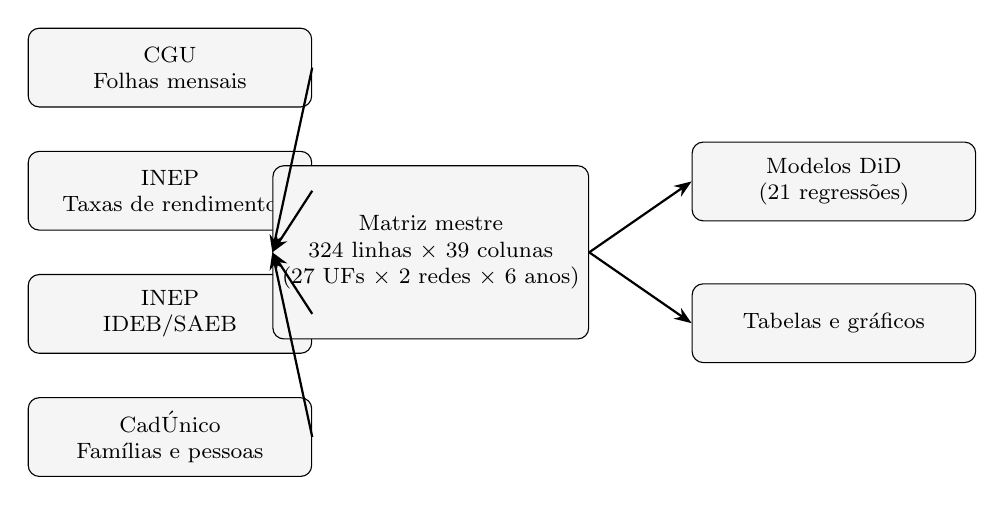
\begin{tikzpicture}[
        node distance=0.55cm and 0.9cm,
        caixa/.style={draw, rounded corners, align=center, font=\footnotesize,
                      minimum width=3.6cm, minimum height=1.0cm, fill=gray!8},
        seta/.style={-{Stealth[length=2.2mm]}, thick}
    ]
        \node[caixa] (cgu)  {CGU\\Folhas mensais};
        \node[caixa, below=of cgu]  (rend) {INEP\\Taxas de rendimento};
        \node[caixa, below=of rend] (ideb) {INEP\\IDEB/SAEB};
        \node[caixa, below=of ideb] (cad)  {CadÚnico\\Famílias e pessoas};

        \node[caixa, right=1.3cm of $(rend)!0.5!(ideb)$, minimum height=2.2cm] (mat)
            {Matriz mestre\\324 linhas $\times$ 39 colunas\\(27 UFs $\times$ 2 redes $\times$ 6 anos)};

        \node[caixa, right=1.3cm of mat, yshift=0.9cm]  (did) {Modelos DiD\\(21 regressões)};
        \node[caixa, right=1.3cm of mat, yshift=-0.9cm] (graf) {Tabelas e gráficos};

        \foreach \n in {cgu, rend, ideb, cad} \draw[seta] (\n.east) -- (mat.west);
        \draw[seta] (mat.east) -- (did.west);
        \draw[seta] (mat.east) -- (graf.west);
    \end{tikzpicture}
    \fonte{Elaborada pelo autor (2026).}
\end{figure}

Na etapa de tratamento, os pacotes mensais da CGU foram lidos integralmente e agregados por UF, mês de folha e tipo de incentivo.
Foram processadas todas as nove competências de 2024 (março a dezembro, inexistindo a folha de julho em razão do recesso escolar), além das folhas de janeiro e fevereiro de 2025, que contêm os depósitos de conclusão e de Enem referentes ao ano letivo de 2024.
As planilhas do INEP foram filtradas para o ensino médio, para o nível de agregação UF e para as dependências administrativas estadual e privada.

As bases foram então integradas em uma matriz mestre balanceada de 324 observações (27 UFs $\times$ 2 redes $\times$ 6 anos: 2019, 2021, 2022, 2023, 2024 e 2025) e 39 colunas, documentada no \autoref{chap_apendice_dicionario}.
Os valores ausentes são estruturais: os indicadores do SAEB e do IDEB existem apenas em anos ímpares, as taxas anuais de rendimento foram consolidadas para 2022 a 2025 e as variáveis financeiras do Pé-de-Meia referem-se exclusivamente às 27 observações da rede estadual em 2024.

\subsection{Auditoria de consistência das folhas de pagamento}
\label{subsec_auditoria}

Durante a coleta, identificou-se que a versão do arquivo de março de 2024 inicialmente obtida continha 4.205.138 parcelas, totalizando R\$ 841.027.600,00.
A versão retificada posteriormente publicada pela CGU contém 2.416.252 parcelas e R\$ 483.250.400,00, uma redução de 1.788.886 registros ($-42{,}54\%$).
A inspeção dos beneficiários maiores de 18 anos, para os quais o NIS é divulgado, mostrou que 68,55\% dos identificadores apresentavam duas linhas idênticas na mesma data de pagamento na versão antiga, o que caracteriza duplicação.
Todas as análises deste trabalho utilizam exclusivamente a versão retificada.

\section{Desidentificação dos dados e variáveis \textit{proxy}}
\label{sec_desidentificacao}

Na folha retificada de março de 2024, 88,86\% dos registros trazem o nome do beneficiário substituído pela expressão ``beneficiário menor de 18 anos'', com CPF e NIS ausentes.
Essa desidentificação decorre das normas de proteção de dados de crianças e adolescentes previstas na LGPD \cite{Brasil2018LGPD} e no ECA \cite{Brasil1990ECA}.
Como consequência, não há chave individual confiável para rastrear um mesmo estudante ao longo das folhas mensais.

Por esse motivo, adotaram-se duas variáveis \textit{proxy}.
Como o Incentivo-Matrícula é pago uma única vez por estudante elegível em cada ano letivo, a contagem de parcelas dessa modalidade em 2024 (4.008.269) foi utilizada como estimativa do número de estudantes beneficiários.
Analogamente, a contagem de parcelas de Incentivo-Conclusão referentes ao ano letivo de 2024 pagas até fevereiro de 2025 (3.037.316) foi utilizada como estimativa do número de estudantes que receberam o depósito de conclusão até essa data.

\section{Análise estatística}
\label{sec_analise_estatistica}

\subsection{Especificação do modelo de Diferenças em Diferenças}
\label{subsec_especificacao}

O grupo tratado é a rede pública estadual ($D_r = 1$), e o grupo de comparação é a rede privada ($D_r = 0$), não elegível ao programa.
O período pós-programa é definido por $\mathit{Post}_t = 1$ para $t \geq 2024$.
A especificação principal é dada pela \autoref{eq_did}:
\begin{equation}
    \label{eq_did}
    Y_{urt} = \alpha_{ur} + \lambda_t + \beta\,(D_r \times \mathit{Post}_t) + \varepsilon_{urt},
\end{equation}
em que $Y_{urt}$ é o desfecho da UF $u$, na rede $r$ e no ano $t$; $\alpha_{ur}$ é o efeito fixo do par UF $\times$ rede, que absorve todas as características invariantes no tempo de cada combinação; $\lambda_t$ é o efeito fixo de ano, que absorve choques comuns às duas redes; e $\beta$ é o coeficiente de interesse, que mede a variação diferencial da rede estadual no período pós-programa.

Os desfechos e as janelas analíticas são os seguintes:
\begin{itemize}
    \item taxas anuais de abandono, aprovação e reprovação do ensino médio, no painel 2022--2025 ($n = 216$);
    \item notas do SAEB em Matemática e Língua Portuguesa, nota padronizada $N$, indicador de rendimento $P$ e IDEB observado, no painel bienal completo 2019--2025 ($n = 216$) e na janela imediata 2023 \textit{versus} 2025 ($n = 108$).
\end{itemize}

\subsection{Testes de pré-tendência}
\label{subsec_pretendencia}

Para avaliar a plausibilidade das tendências paralelas, estimou-se, restrito ao período pré-programa, o modelo da \autoref{eq_pretendencia}:
\begin{equation}
    \label{eq_pretendencia}
    Y_{urt} = \alpha_{ur} + \lambda_t + \sum_{k \in \mathcal{K}} \theta_k\,\big(D_r \times \mathbf{1}[t = k]\big) + \varepsilon_{urt},
\end{equation}
em que $\mathcal{K} = \{2023\}$ para as taxas de rendimento (referência: 2022) e $\mathcal{K} = \{2021, 2023\}$ para os indicadores do SAEB e do IDEB (referência: 2019).
Sob tendências paralelas, espera-se $\theta_k = 0$ para todo $k$.

\subsection{Inferência}
\label{subsec_inferencia}

Os modelos foram estimados por Mínimos Quadrados Ordinários, com erros-padrão robustos agrupados por UF ($G = 27$ \textit{clusters}), o que acomoda a correlação serial e a correlação entre as duas redes de uma mesma UF \cite{Bertrand2004}.
Dado o número reduzido de \textit{clusters}, os testes de hipótese utilizam a distribuição $t$ de Student com $G - 1 = 26$ graus de liberdade \cite{Cameron2015}.

No total, foram estimados 21 modelos, que produzem 26 testes de hipótese sobre coeficientes de interação: 13 testes DiD pós-programa (3 de fluxo anual, 5 no painel bienal completo e 5 na janela imediata) e 13 testes de pré-tendência.
Para controlar a taxa de erro do tipo I decorrente da multiplicidade de testes, os resultados são também confrontados com o limiar de Bonferroni \cite{Dunn1961}, definido pela \autoref{eq_bonferroni}:
\begin{equation}
    \label{eq_bonferroni}
    \alpha_{\text{Bonf}} = \frac{\alpha}{m},
\end{equation}
em que $\alpha = 0{,}05$ e $m$ é o número de testes da família considerada.
Para os 13 testes DiD, $\alpha_{\text{Bonf}} \approx 0{,}0038$; para os 5 desfechos da janela imediata, $\alpha_{\text{Bonf}} = 0{,}0100$.
Como análise de robustez, os modelos foram também estimados em uma especificação preliminar sem efeitos fixos de unidade e com distribuição normal, cujos resultados constam no \autoref{chap_apendice_comparacao}.
              % Metodologia
% ------------------------------------------------------------------------------
% Resultados e discussão
% ------------------------------------------------------------------------------

\chapter{Resultados e discussão}
\label{chap_resultados}

Este capítulo apresenta os resultados em quatro etapas.
A \autoref{sec_execucao_financeira} descreve a execução financeira do Pé-de-Meia em 2024.
A \autoref{sec_series_descritivas} apresenta a evolução descritiva dos indicadores educacionais por rede.
A \autoref{sec_estimativas_did} reporta as estimativas de Diferenças em Diferenças e os testes de pré-tendência.
Por fim, a \autoref{sec_discussao} discute os resultados à luz da literatura e das limitações do delineamento.
Em todas as tabelas e figuras, as médias por rede correspondem à média simples das 27 UFs, coerente com a ponderação implícita dos modelos em painel.

% ------------------------------------------------------------------------------
\section{Execução financeira do Pé-de-Meia em 2024}
\label{sec_execucao_financeira}

A \autoref{tab_execucao_mensal} apresenta a execução mensal nacional do programa no exercício de 2024.
O montante transferido cresce ao longo do ano, passando de R\$ 483,3 milhões na primeira folha para valores próximos de R\$ 686 milhões nos meses finais, em razão da incorporação progressiva de novos beneficiários.
O exercício totalizou R\$ 5.587.440.225,00 em 27.892.528 parcelas.

\begin{table}[!htb]
    \centering
    \caption{Execução mensal nacional do Pé-de-Meia no exercício de 2024}
    \label{tab_execucao_mensal}
    \small
    \begin{tabularx}{\textwidth}{cXrr}
        \toprule
        \textbf{Folha} & \textbf{Observação operacional} & \textbf{Valor (R\$)} & \textbf{Parcelas} \\
        \midrule
        03/2024 & 1º lote de matrícula (versão retificada) & 483.250.400,00 & 2.416.252 \\
        04/2024 & 1ª parcela de frequência e matrícula complementar & 552.561.000,00 & 2.762.805 \\
        05/2024 & 2ª parcela de frequência e matrícula complementar & 549.488.000,00 & 2.747.440 \\
        06/2024 & 3ª parcela de frequência e matrícula complementar & 659.172.000,00 & 3.295.860 \\
        08/2024 & Retomada pós-recesso e expansão do público & 630.427.600,00 & 3.152.138 \\
        09/2024 & Parcela regular & 656.487.400,00 & 3.282.437 \\
        10/2024 & Parcela regular & 686.305.175,00 & 3.418.224 \\
        11/2024 & Parcela regular & 683.902.550,00 & 3.404.749 \\
        12/2024 & Última folha do exercício & 685.846.100,00 & 3.412.623 \\
        \midrule
        \multicolumn{2}{l}{\textbf{Total do exercício de 2024 (9 folhas)}} & \textbf{5.587.440.225,00} & \textbf{27.892.528} \\
        \bottomrule
    \end{tabularx}
    \fonte{Elaborada pelo autor (2026) com dados de \citeonline{CGU2026PeDeMeia}. Não há folha em julho, em razão do recesso escolar.}
\end{table}

Ao exercício de 2024 somam-se os depósitos de conclusão (3.037.316 parcelas; R\$ 3,04 bilhões) e de Enem (450.679 parcelas; R\$ 90,1 milhões) referentes ao ano letivo de 2024, pagos na folha de fevereiro de 2025.
O custo do ciclo letivo de 2024 contabilizado até fevereiro de 2025 é, portanto, de R\$ 8.714.892.025,00, valor que deve ser interpretado como um \textit{piso}, pois a folha de março de 2025 ainda contém pagamentos retroativos de conclusão do ano letivo de 2024 (ao menos 111.734 parcelas nas 16 UFs disponíveis no arquivo parcial analisado).
Dividido pelas 4.008.269 parcelas de matrícula (\textit{proxy} de estudantes beneficiários), esse piso corresponde a R\$ 2.174,23 por estudante.

A \autoref{fig_repasses_uf} apresenta a distribuição dos repasses de 2024 por pessoa cadastrada no CadÚnico em cada UF.
Observa-se um claro gradiente regional: as UFs do Nordeste e do Norte concentram os maiores valores relativos, liderados por Maranhão (R\$ 79,54) e Pará (R\$ 78,93), enquanto as UFs do Sul e do Sudeste ocupam as últimas posições, com Rio Grande do Sul (R\$ 38,94) e Paraná (R\$ 41,00).
A razão nacional agregada é de R\$ 58,61 por pessoa cadastrada.
Esse padrão é compatível com a maior proporção de jovens de famílias de baixa renda matriculados no ensino médio público nessas regiões.
Alagoas, com R\$ 72,86 por pessoa cadastrada, situa-se na quarta posição nacional.
A tabela completa por UF encontra-se no \autoref{chap_apendice_uf}.

\begin{figure}[!htb]
    \centering
    \caption{Repasses do Pé-de-Meia por pessoa cadastrada no CadÚnico, por UF (exercício de 2024)}
    \label{fig_repasses_uf}
    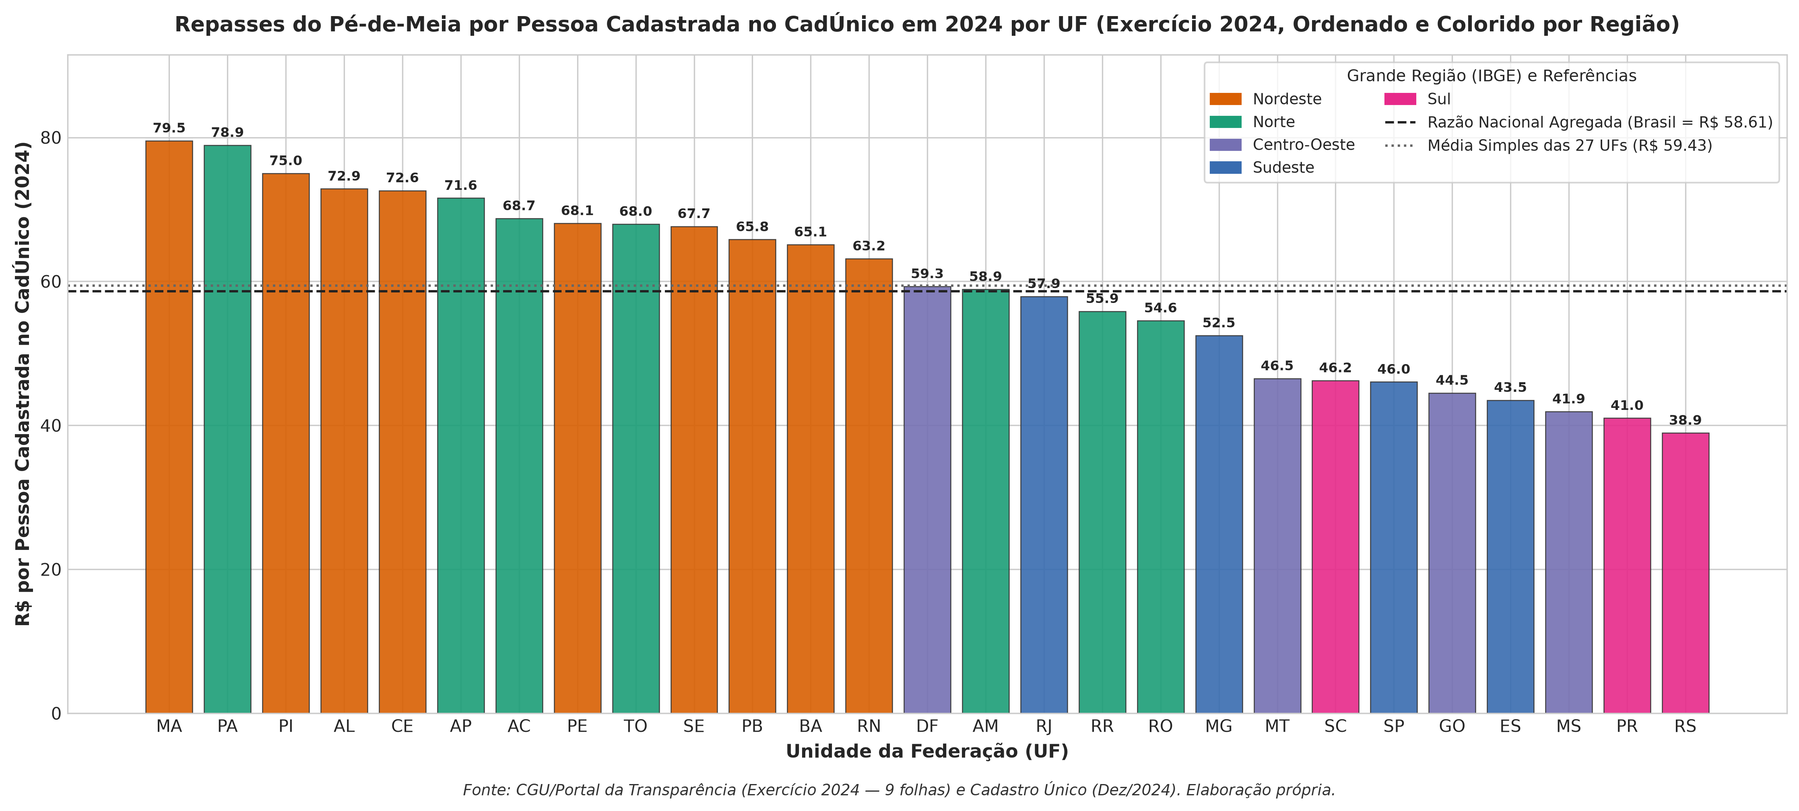
\includegraphics[width=\textwidth]{figuras/grafico_repasses_pedemeia_uf_nacional}
    \fonte{Elaborada pelo autor (2026) com dados de \citeonline{CGU2026PeDeMeia} e \citeonline{Alagoas2026CadUnico}.}
\end{figure}

O custo por estudante (\textit{proxy}) no exercício de 2024 foi de R\$ 1.393,98 no agregado nacional, variando de R\$ 1.133,91 no Amazonas a R\$ 1.566,76 no Pará.
Na folha de fevereiro de 2025, a razão entre parcelas de conclusão e total de pagamentos de 2024 foi de 10,89\% no agregado nacional, mas atipicamente baixa no Amapá (4,03\%) e em Santa Catarina (2,84\%).
No caso do Amapá, verificou-se nos microdados de março de 2025 que outras 10.797 parcelas de conclusão do ano letivo de 2024 foram pagas nessa folha, o que comprova o pagamento defasado.
Para Santa Catarina, cuja UF não consta no arquivo parcial disponível, formula-se a mesma hipótese.
Por essa razão, as comparações financeiras entre UFs utilizam exclusivamente o exercício fechado de 2024.

% ------------------------------------------------------------------------------
\section{Evolução descritiva dos indicadores educacionais}
\label{sec_series_descritivas}

\subsection{Taxas de rendimento escolar}
\label{subsec_resultados_rendimento}

A \autoref{tab_taxas_rendimento} e a \autoref{fig_taxas_rendimento} apresentam a evolução das taxas de rendimento do ensino médio por rede entre 2022 e 2025.
A taxa média de abandono da rede estadual caiu de 7,09\% em 2022 para 2,51\% em 2025, enquanto na rede privada passou de 0,88\% para 0,36\%.
Em consequência, o hiato de abandono entre as redes reduziu-se de 6,21 para 2,14 pontos percentuais.

Contudo, a maior parte dessa convergência ocorreu entre 2022 e 2023, \textit{antes} da implantação do programa: nesse intervalo, o abandono estadual recuou 3,08 p.p., contra apenas 0,11 p.p. na rede privada.
Esse movimento é compatível com a recuperação pós-pandemia e antecipa o principal desafio de identificação discutido na \autoref{sec_estimativas_did}.

\begin{table}[!htb]
    \centering
    \caption{Taxas de rendimento do ensino médio por rede (média simples das 27 UFs, em \%)}
    \label{tab_taxas_rendimento}
    \small
    \begin{tabular}{lccccccc}
        \toprule
        & \multicolumn{2}{c}{\textbf{Aprovação}} & \multicolumn{2}{c}{\textbf{Reprovação}} & \multicolumn{2}{c}{\textbf{Abandono}} & \textbf{Hiato de} \\
        \cmidrule(lr){2-3} \cmidrule(lr){4-5} \cmidrule(lr){6-7}
        \textbf{Ano} & Estadual & Privada & Estadual & Privada & Estadual & Privada & \textbf{abandono} \\
        \midrule
        2022 & 84,12 & 96,62 & 8,79 & 2,50 & 7,09 & 0,88 & 6,21 \\
        2023 & 89,78 & 96,85 & 6,21 & 2,39 & 4,01 & 0,77 & 3,24 \\
        2024 & 90,07 & 97,26 & 6,20 & 2,19 & 3,73 & 0,55 & 3,18 \\
        2025 & 93,80 & 97,61 & 3,70 & 2,02 & 2,51 & 0,36 & 2,14 \\
        \midrule
        $\Delta$ 2022--2023 (pré) & $+5{,}66$ & $+0{,}23$ & $-2{,}58$ & $-0{,}12$ & $-3{,}08$ & $-0{,}11$ & $-2{,}97$ \\
        $\Delta$ pós $-$ pré\textsuperscript{a} & $+4{,}99$ & $+0{,}70$ & $-2{,}55$ & $-0{,}34$ & $-2{,}43$ & $-0{,}37$ & $-2{,}07$ \\
        \bottomrule
    \end{tabular}
    \fonte{Elaborada pelo autor (2026) com dados de \citeonline{INEP2026Rendimento}. \textsuperscript{a}Média de 2024--2025 menos média de 2022--2023. Hiato = Estadual $-$ Privada, em p.p.}
\end{table}

\begin{figure}[!htb]
    \centering
    \caption{Taxas médias de abandono e de aprovação no ensino médio por rede (2022--2025)}
    \label{fig_taxas_rendimento}
    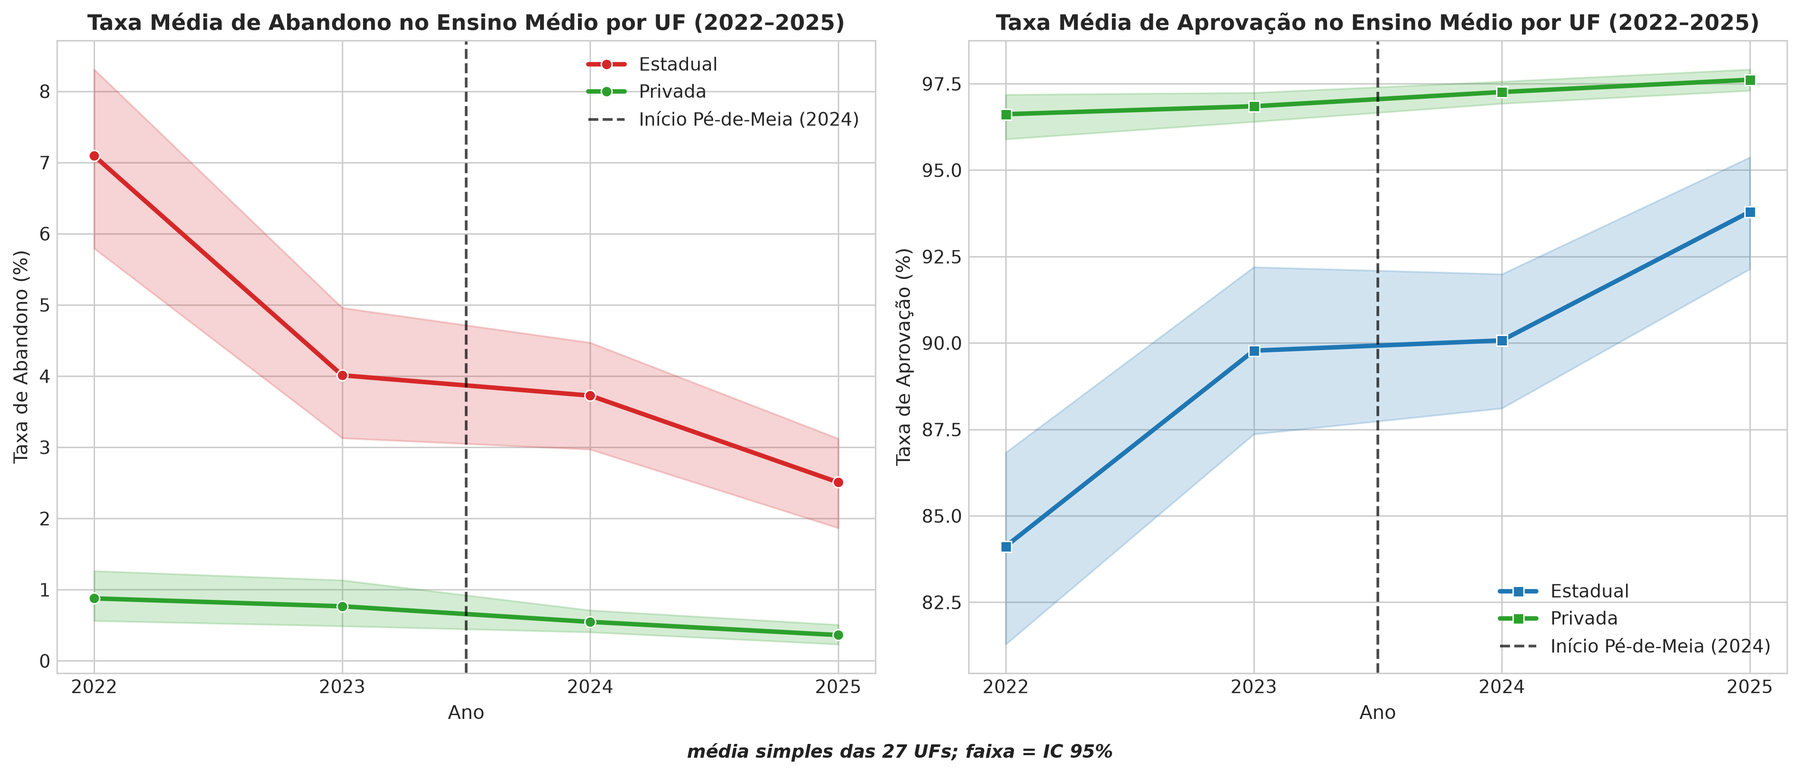
\includegraphics[width=\textwidth]{figuras/grafico_taxas_rendimento_2025}
    \fonte{Elaborada pelo autor (2026) com dados de \citeonline{INEP2026Rendimento}. Média simples das 27 UFs; a faixa sombreada representa o intervalo de confiança de 95\%.}
\end{figure}

Observa-se ainda que a rede privada já operava, em 2022, próxima dos limites da escala percentual, com aprovação de 96,62\% e abandono de 0,88\%.
Formula-se, assim, a hipótese de \textit{compressão assintótica}: como a rede privada dispõe de pouca margem para melhorar, qualquer recuperação expressiva da rede estadual se traduz mecanicamente em convergência entre as redes, independentemente da existência de uma intervenção específica.

\subsection{Desempenho no SAEB e IDEB}
\label{subsec_resultados_ideb}

A \autoref{fig_ideb_matematica} apresenta a evolução da nota do SAEB em Matemática e do IDEB por rede.
Entre 2019 e 2021, ambas as redes sofreram perdas de proficiência associadas à pandemia, mais acentuadas na rede privada (de 331,17 para 316,58 pontos em Matemática) do que na estadual (de 266,21 para 261,11 pontos).
Essa assimetria já produz uma aproximação entre as redes antes do programa.

\begin{figure}[!htb]
    \centering
    \caption{Evolução da nota do SAEB em Matemática e do IDEB do ensino médio por rede (2019--2025)}
    \label{fig_ideb_matematica}
    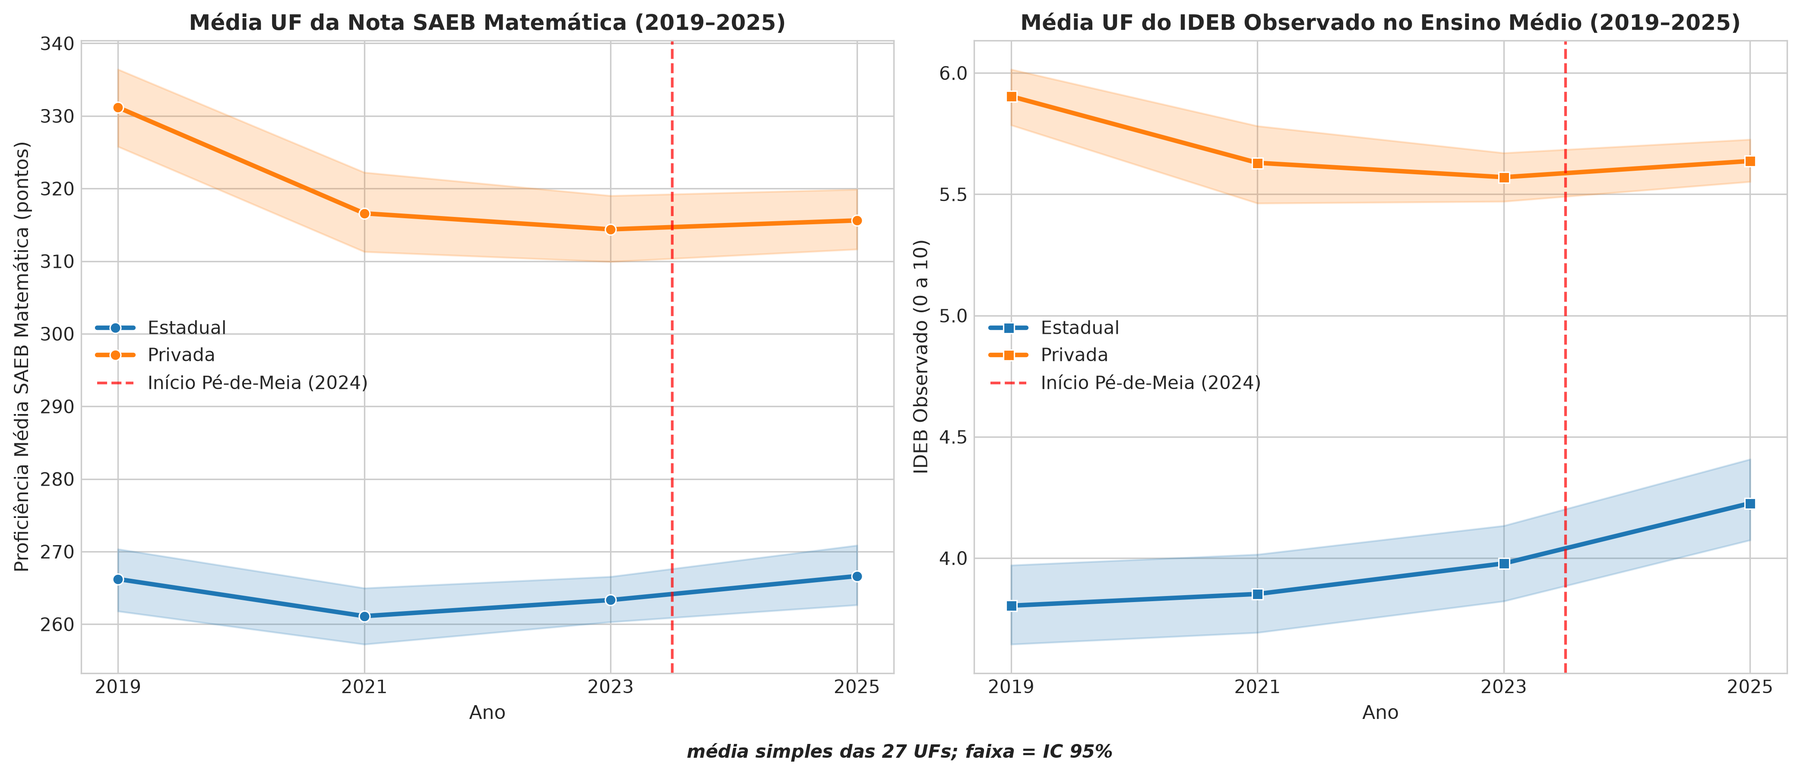
\includegraphics[width=\textwidth]{figuras/grafico_ideb_matematica_evolucao}
    \fonte{Elaborada pelo autor (2026) com dados de \citeonline{INEP2026IDEB}. Média simples das 27 UFs; a faixa sombreada representa o intervalo de confiança de 95\%.}
\end{figure}

A \autoref{tab_decomposicao_ideb} detalha a evolução do IDEB e de seus componentes.
Entre 2023 e 2025, o IDEB estadual avançou 0,2481 ponto, contra 0,0667 na rede privada.
Pela decomposição da \autoref{eq_decomposicao}, a contribuição do fluxo escolar na rede estadual é de aproximadamente $\bar{N}\,\Delta P \approx 4{,}44 \times 0{,}0377 = 0{,}167$ ponto, ou 67,5\% do ganho total.
Assim, cerca de dois terços do avanço do IDEB estadual no período decorrem da melhoria das taxas de aprovação, e não da proficiência.

\begin{table}[!htb]
    \centering
    \caption{Evolução do SAEB, dos componentes $N$ e $P$ e do IDEB do ensino médio por rede (média simples das 27 UFs)}
    \label{tab_decomposicao_ideb}
    \small
    \begin{tabular}{llrrrrr}
        \toprule
        \textbf{Indicador} & \textbf{Rede} & \textbf{2019} & \textbf{2021} & \textbf{2023} & \textbf{2025} & \textbf{$\Delta$ 2023--2025} \\
        \midrule
        \multirow{2}{*}{SAEB Matemática} & Estadual & 266,21 & 261,11 & 263,33 & 266,63 & $+3{,}30$ \\
                                          & Privada  & 331,17 & 316,58 & 314,38 & 315,61 & $+1{,}23$ \\
        \addlinespace
        \multirow{2}{*}{SAEB Língua Portuguesa} & Estadual & 269,09 & 267,53 & 267,83 & 270,71 & $+2{,}88$ \\
                                                 & Privada  & 319,97 & 310,75 & 311,26 & 310,68 & $-0{,}58$ \\
        \addlinespace
        \multirow{2}{*}{Nota padronizada ($N$)} & Estadual & 4,4567 & 4,3618 & 4,3974 & 4,4869 & $+0{,}0895$ \\
                                                 & Privada  & 6,1307 & 5,7879 & 5,7646 & 5,7731 & $+0{,}0085$ \\
        \addlinespace
        \multirow{2}{*}{Indicador de rendimento ($P$)} & Estadual & 0,8503 & 0,8828 & 0,9037 & 0,9414 & $+0{,}0377$ \\
                                                        & Privada  & 0,9628 & 0,9721 & 0,9663 & 0,9778 & $+0{,}0116$ \\
        \addlinespace
        \multirow{2}{*}{IDEB ($N \times P$)} & Estadual & 3,8037 & 3,8519 & 3,9778 & 4,2259 & $+0{,}2481$ \\
                                              & Privada  & 5,9037 & 5,6296 & 5,5704 & 5,6370 & $+0{,}0667$ \\
        \bottomrule
    \end{tabular}
    \fonte{Elaborada pelo autor (2026) com dados de \citeonline{INEP2026IDEB}.}
\end{table}

% ------------------------------------------------------------------------------
\section{Estimativas de Diferenças em Diferenças}
\label{sec_estimativas_did}

\subsection{Associações no período pós-programa}
\label{subsec_did_pos}

A \autoref{tab_did_pos} reporta os 13 coeficientes DiD estimados pela \autoref{eq_did}.
Nas taxas anuais de rendimento, a rede estadual apresentou, em relação à privada, redução diferencial de 2,07 p.p. no abandono, aumento de 4,28 p.p. na aprovação e redução de 2,21 p.p. na reprovação no período 2024--2025, todos significativos inclusive após a correção de Bonferroni.

No painel bienal completo (2019--2025), todos os indicadores do SAEB e do IDEB apresentam coeficientes positivos e significativos.
Entretanto, essas estimativas comparam o período pós-programa com uma média que inclui 2019, ano anterior às perdas pandêmicas assimétricas descritas na \autoref{subsec_resultados_ideb}, e estão, portanto, contaminadas pela divergência pré-existente entre as redes.

Na janela imediata (2023 \textit{versus} 2025), que isola a transição em torno da implantação, as notas do SAEB em Matemática ($p = 0{,}3814$) e em Língua Portuguesa ($p = 0{,}0817$) e a nota padronizada $N$ ($p = 0{,}1830$) deixam de ser significativas ao nível de 5\%.
O indicador de rendimento $P$ apresenta significância limítrofe ($p = 0{,}0505$), e o IDEB, coeficiente de $+0{,}1815$ ($p = 0{,}0115$), valor que não supera o limiar de Bonferroni para os cinco desfechos da janela ($\alpha_{\text{Bonf}} = 0{,}0100$).
Esse resultado deve, portanto, ser considerado apenas \textit{sugestivo} e interpretado em conjunto com seus componentes: o avanço do IDEB reflete sobretudo o fluxo escolar ($P$), sem ganho estatisticamente significativo de proficiência ($N$).

\begin{table}[!htb]
    \centering
    \caption{Estimativas de Diferenças em Diferenças no período pós-programa (efeitos fixos de UF $\times$ rede e de ano)}
    \label{tab_did_pos}
    \small
    \begin{tabular}{llcrrrr}
        \toprule
        \textbf{Desfecho} & \textbf{Janela} & \textbf{$n$} & \textbf{$\hat{\beta}$} & \textbf{EP} & \textbf{$t$} & \textbf{Valor-$p$} \\
        \midrule
        \multicolumn{7}{l}{\textit{Painel A -- Taxas anuais de rendimento (p.p.)}} \\
        Abandono   & 2022--2025 & 216 & $-2{,}0685$ & 0,3477 & $-5{,}949$ & $<0{,}0001$\textsuperscript{\dag} \\
        Aprovação  & 2022--2025 & 216 & $+4{,}2833$ & 0,7980 & $+5{,}368$ & $<0{,}0001$\textsuperscript{\dag} \\
        Reprovação & 2022--2025 & 216 & $-2{,}2148$ & 0,5958 & $-3{,}718$ & $0{,}0010$\textsuperscript{\dag} \\
        \addlinespace
        \multicolumn{7}{l}{\textit{Painel B -- Painel bienal completo}} \\
        SAEB Matemática (pts)        & 2019--2025 & 216 & $+8{,}1802$ & 2,0593 & $+3{,}972$ & $0{,}0005$\textsuperscript{\dag} \\
        SAEB Língua Portuguesa (pts) & 2019--2025 & 216 & $+5{,}8777$ & 1,7242 & $+3{,}409$ & $0{,}0021$\textsuperscript{\dag} \\
        Nota padronizada ($N$)       & 2019--2025 & 216 & $+0{,}2029$ & 0,0530 & $+3{,}825$ & $0{,}0007$\textsuperscript{\dag} \\
        Indicador de rendimento ($P$) & 2019--2025 & 216 & $+0{,}0517$ & 0,0112 & $+4{,}623$ & $0{,}0001$\textsuperscript{\dag} \\
        IDEB ($N \times P$)          & 2019--2025 & 216 & $+0{,}4123$ & 0,0731 & $+5{,}639$ & $<0{,}0001$\textsuperscript{\dag} \\
        \addlinespace
        \multicolumn{7}{l}{\textit{Painel C -- Janela imediata}} \\
        SAEB Matemática (pts)        & 2023 \textit{vs.} 2025 & 108 & $+2{,}0719$ & 2,3270 & $+0{,}890$ & $0{,}3814$ \\
        SAEB Língua Portuguesa (pts) & 2023 \textit{vs.} 2025 & 108 & $+3{,}4641$ & 1,9126 & $+1{,}811$ & $0{,}0817$ \\
        Nota padronizada ($N$)       & 2023 \textit{vs.} 2025 & 108 & $+0{,}0810$ & 0,0592 & $+1{,}368$ & $0{,}1830$ \\
        Indicador de rendimento ($P$) & 2023 \textit{vs.} 2025 & 108 & $+0{,}0261$ & 0,0127 & $+2{,}051$ & $0{,}0505$ \\
        IDEB ($N \times P$)          & 2023 \textit{vs.} 2025 & 108 & $+0{,}1815$ & 0,0668 & $+2{,}718$ & $0{,}0115$ \\
        \bottomrule
    \end{tabular}
    \fonte{Elaborada pelo autor (2026). Erros-padrão agrupados por UF ($G = 27$); valores-$p$ da distribuição $t$ com 26 graus de liberdade. \textsuperscript{\dag}Significativo após correção de Bonferroni para os 13 testes DiD ($\alpha_{\text{Bonf}} \approx 0{,}0038$).}
\end{table}

\subsection{Testes de pré-tendência}
\label{subsec_resultados_pretendencia}

A \autoref{tab_pretendencia} apresenta os 13 coeficientes de pré-tendência estimados pela \autoref{eq_pretendencia}.
A hipótese de tendências paralelas é rejeitada ao nível de 5\% em 11 dos 13 testes.
Nas taxas de rendimento, a rede estadual já apresentava, entre 2022 e 2023, redução diferencial de 2,97 p.p. no abandono ($p = 0{,}0031$) e aumento de 5,43 p.p. na aprovação ($p = 0{,}0144$), magnitudes superiores às próprias estimativas DiD pós-programa.
Nos indicadores do SAEB e do IDEB, a divergência entre 2019 e 2023 é significativa em todos os desfechos ($p \leq 0{,}0010$).
As exceções são a taxa de reprovação entre 2022 e 2023, marginalmente significativa ao nível de 10\% ($p = 0{,}0642$), e o indicador de rendimento $P$ entre 2019 e 2021 ($p = 0{,}2284$).

\begin{table}[!htb]
    \centering
    \caption{Testes de pré-tendência (efeitos fixos de UF $\times$ rede e de ano)}
    \label{tab_pretendencia}
    \small
    \begin{tabular}{llcrrrr}
        \toprule
        \textbf{Desfecho} & \textbf{Comparação} & \textbf{$n$} & \textbf{$\hat{\theta}_k$} & \textbf{EP} & \textbf{$t$} & \textbf{Valor-$p$} \\
        \midrule
        Abandono (p.p.)              & 2022 \textit{vs.} 2023 & 108 & $-2{,}9704$ & 0,9106 & $-3{,}262$ & $0{,}0031$ \\
        Aprovação (p.p.)             & 2022 \textit{vs.} 2023 & 108 & $+5{,}4296$ & 2,0696 & $+2{,}623$ & $0{,}0144$ \\
        Reprovação (p.p.)            & 2022 \textit{vs.} 2023 & 108 & $-2{,}4593$ & 1,2724 & $-1{,}933$ & $0{,}0642$ \\
        \addlinespace
        SAEB Matemática (pts)        & 2019 \textit{vs.} 2021 & 162 & $+9{,}4881$  & 2,0109 & $+4{,}718$ & $0{,}0001$ \\
                                     & 2019 \textit{vs.} 2023 & 162 & $+13{,}9067$ & 2,2676 & $+6{,}133$ & $<0{,}0001$ \\
        SAEB Língua Portuguesa (pts) & 2019 \textit{vs.} 2021 & 162 & $+7{,}6607$  & 1,6716 & $+4{,}583$ & $0{,}0001$ \\
                                     & 2019 \textit{vs.} 2023 & 162 & $+7{,}4507$  & 1,8328 & $+4{,}065$ & $0{,}0004$ \\
        Nota padronizada ($N$)       & 2019 \textit{vs.} 2021 & 162 & $+0{,}2479$  & 0,0513 & $+4{,}833$ & $0{,}0001$ \\
                                     & 2019 \textit{vs.} 2023 & 162 & $+0{,}3069$  & 0,0577 & $+5{,}322$ & $<0{,}0001$ \\
        Indicador de rendimento ($P$) & 2019 \textit{vs.} 2021 & 162 & $+0{,}0233$ & 0,0189 & $+1{,}233$ & $0{,}2284$ \\
                                     & 2019 \textit{vs.} 2023 & 162 & $+0{,}0500$  & 0,0134 & $+3{,}719$ & $0{,}0010$ \\
        IDEB ($N \times P$)          & 2019 \textit{vs.} 2021 & 162 & $+0{,}3222$  & 0,1027 & $+3{,}136$ & $0{,}0042$ \\
                                     & 2019 \textit{vs.} 2023 & 162 & $+0{,}5074$  & 0,0901 & $+5{,}634$ & $<0{,}0001$ \\
        \bottomrule
    \end{tabular}
    \fonte{Elaborada pelo autor (2026). Erros-padrão agrupados por UF ($G = 27$); valores-$p$ da distribuição $t$ com 26 graus de liberdade. Anos de referência: 2022 (rendimento) e 2019 (SAEB/IDEB).}
\end{table}

A \autoref{fig_diferenca_redes} sintetiza visualmente esse diagnóstico.
O hiato de abandono cai de 6,21 p.p. em 2022 para 3,24 p.p. em 2023, permanece praticamente estável em 2024 (3,18 p.p.) e recua para 2,14 p.p. em 2025.
Na Matemática, a diferença entre as redes diminui continuamente desde 2019 ($-64{,}96$ pontos) até 2025 ($-48{,}98$ pontos), sem inflexão visível no ano de implantação do programa.

\begin{figure}[!htb]
    \centering
    \caption{Diferença Estadual $-$ Privada na taxa de abandono (2022--2025) e na nota do SAEB em Matemática (2019--2025)}
    \label{fig_diferenca_redes}
    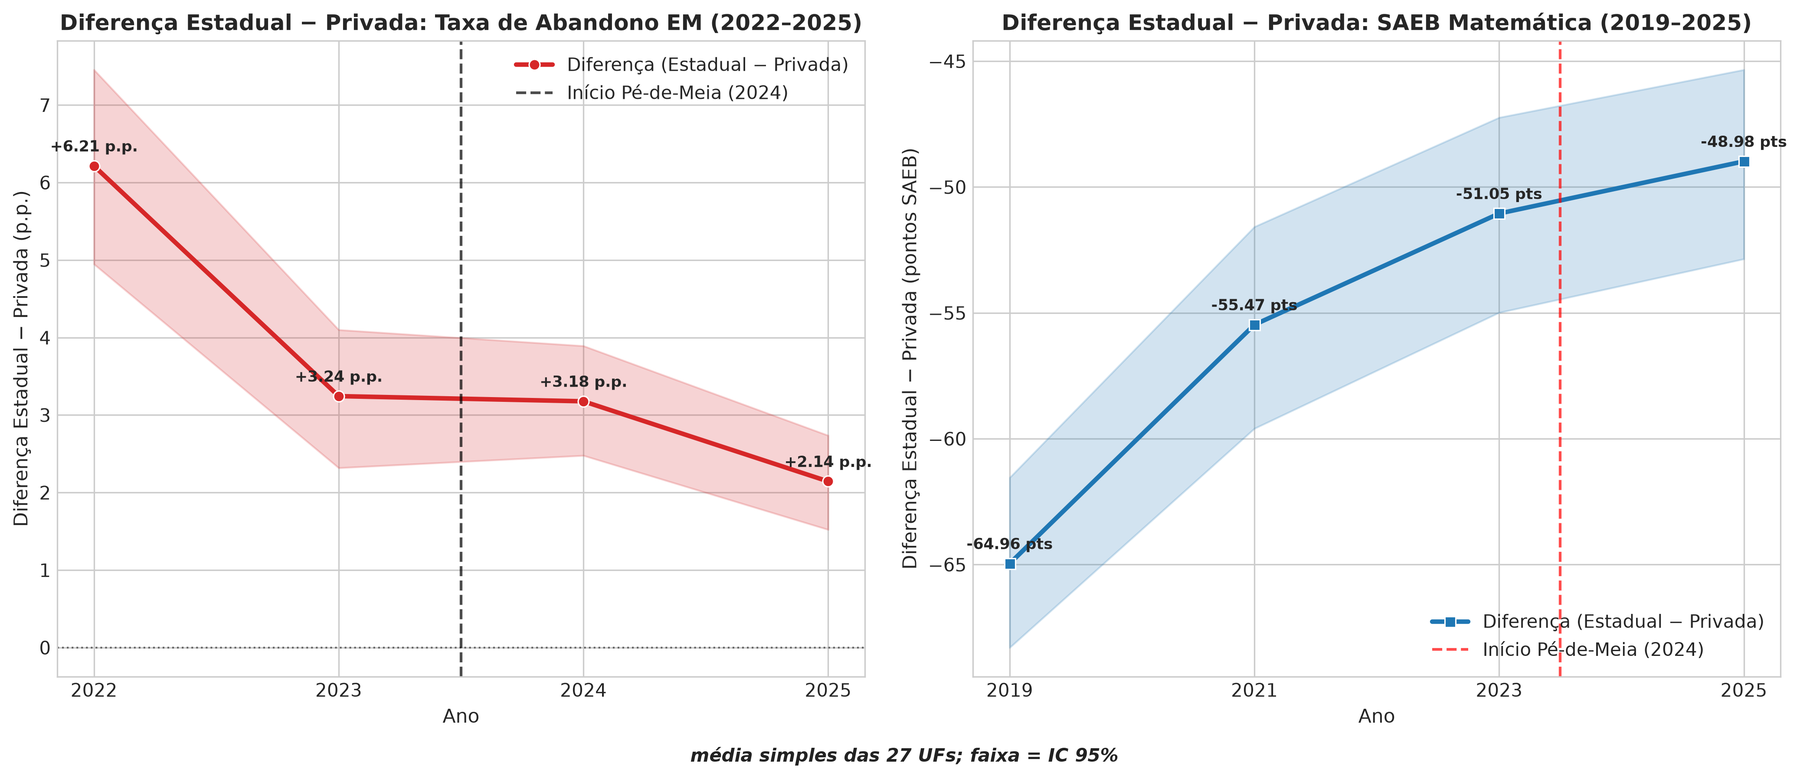
\includegraphics[width=\textwidth]{figuras/grafico_diferenca_estadual_privada}
    \fonte{Elaborada pelo autor (2026) com dados de \citeonline{INEP2026Rendimento} e \citeonline{INEP2026IDEB}. Média simples das 27 UFs; a faixa sombreada representa o intervalo de confiança de 95\%.}
\end{figure}

\subsection{Cenários exploratórios de custo}
\label{subsec_cenarios_custo}

Como as tendências paralelas são rejeitadas, a fração da associação de $-2{,}07$ p.p. no abandono efetivamente atribuível ao programa é desconhecida.
A \autoref{tab_cenarios_custo} apresenta, em caráter estritamente exploratório, o custo nacional por ponto percentual de redução do abandono sob diferentes hipóteses de atribuição, tomando como base o piso do custo do ciclo de 2024 (R\$ 8,71 bilhões).
O cenário de 100\% representa apenas um teto teórico.

\begin{table}[!htb]
    \centering
    \caption{Cenários exploratórios de custo por ponto percentual de redução do abandono (ciclo de 2024, piso)}
    \label{tab_cenarios_custo}
    \small
    \begin{tabular}{ccc}
        \toprule
        \textbf{Atribuição sobre $|\hat{\beta}|$} & \textbf{Redução atribuída (p.p.)} & \textbf{Custo nacional (R\$ bilhões por p.p.)} \\
        \midrule
        100\% (teto teórico) & 2,07 & 4,21 ou mais \\
        50\%                 & 1,03 & 8,43 ou mais \\
        25\%                 & 0,52 & 16,85 ou mais \\
        0\%                  & 0,00 & Não aplicável \\
        \bottomrule
    \end{tabular}
    \fonte{Elaborada pelo autor (2026). Custo do ciclo de 2024 contabilizado até fevereiro de 2025 (R\$ 8.714.892.025,00), interpretado como piso.}
\end{table}

% ------------------------------------------------------------------------------
\section{Discussão}
\label{sec_discussao}

Os resultados apresentam um padrão qualitativamente coerente com a literatura sobre transferências condicionadas: associações expressivas nos indicadores de fluxo escolar (abandono, aprovação e reprovação) e ausência de ganho robusto na proficiência \cite{Fiszbein2009,Glewwe2012}.
A decomposição do IDEB reforça esse padrão, ao mostrar que dois terços do avanço estadual entre 2023 e 2025 decorrem do componente de rendimento.
Esse resultado é consistente com o desenho do Pé-de-Meia, cujos incentivos estão vinculados à matrícula, à frequência e à aprovação, e não ao desempenho em avaliações.

Entretanto, quatro limitações impedem a interpretação causal das estimativas.

\textbf{Violação das tendências paralelas.}
A rejeição da hipótese nula em 11 dos 13 testes de pré-tendência indica que as redes já convergiam antes do programa, impulsionadas pela recuperação pós-pandemia e, possivelmente, pela compressão assintótica da rede privada.
Essa convergência compromete não apenas as janelas longas, mas também a janela imediata, pois não é possível separar empiricamente a continuidade inercial da convergência de uma eventual contribuição do programa \cite{Roth2023}.

\textbf{Multiplicidade de testes.}
Foram realizados 26 testes na especificação principal.
Sob a correção de Bonferroni, nenhum coeficiente da janela imediata permanece significativo, incluindo o IDEB ($p = 0{,}0115$) \cite{Dunn1961}.

\textbf{Agregação ecológica.}
Nem todos os alunos da rede estadual são elegíveis ao programa, de modo que as estimativas correspondem a uma associação em nível de rede, análoga a uma intenção de tratar ecológica.
Inferências sobre o comportamento individual dos beneficiários estão sujeitas à falácia ecológica \cite{Robinson1950}.

\textbf{Políticas concomitantes e variáveis \textit{proxy}.}
No mesmo período, diversas UFs implementaram políticas de busca ativa e de recomposição da aprendizagem que podem afetar os mesmos desfechos.
Além disso, as contagens de beneficiários baseiam-se em \textit{proxies} derivadas das parcelas de pagamento, e o custo do ciclo de 2024 constitui apenas um piso.

Em síntese, os dados agregados disponíveis são compatíveis com uma contribuição do Pé-de-Meia para a melhoria do fluxo escolar, mas não permitem distingui-la da tendência de convergência já em curso.
               % Resultados e discussão
% ------------------------------------------------------------------------------
% Conclusão
% ------------------------------------------------------------------------------

\chapter{Conclusão}
\label{chap_conclusao}

Este trabalho avaliou, por meio de um delineamento observacional de Diferenças em Diferenças em painel nacional, a associação entre a implantação do Programa Pé-de-Meia e a evolução dos indicadores do ensino médio nas 27 Unidades da Federação entre 2019 e 2025.
Para isso, construiu-se um \textit{pipeline} reprodutível que integra os microdados de pagamento da CGU, as taxas de rendimento do Censo Escolar e os resultados do SAEB e do IDEB, consolidados em uma matriz mestre de 324 observações e 39 variáveis.

Os objetivos propostos foram atingidos.
A auditoria da execução financeira consolidou R\$ 5,59 bilhões transferidos em 2024, documentou a retificação de 1,79 milhão de registros duplicados na folha de março de 2024 e estabeleceu um piso de R\$ 8,71 bilhões para o custo do ciclo letivo de 2024.
A análise distributiva evidenciou maior intensidade relativa dos repasses nas regiões Nordeste e Norte.

Do ponto de vista econométrico, a rede pública estadual apresentou, em relação à privada, redução diferencial de 2,07 pontos percentuais na taxa de abandono e aumento de 4,28 p.p. na taxa de aprovação no período pós-programa, associações robustas à correção para múltiplos testes.
Na janela imediata 2023 \textit{versus} 2025, o avanço do IDEB estadual mostrou-se apenas sugestivo e explicado majoritariamente pelo componente de fluxo escolar, sem ganho significativo de proficiência.

A principal conclusão, contudo, é de natureza metodológica: os testes formais rejeitam a hipótese de tendências paralelas em 11 de 13 casos, revelando que as redes estadual e privada já convergiam antes do programa.
Por essa razão, os resultados não autorizam inferências causais e devem ser lidos como associações descritivas.
Essa constatação é, em si, relevante para o debate público, pois evidencia que comparações simples entre redes ou entre períodos tendem a superestimar a contribuição do programa.

\section{Trabalhos futuros}
\label{sec_trabalhos_futuros}

Como extensões deste trabalho, propõem-se:

\begin{enumerate}
    \item aplicar a análise de sensibilidade de \citeonline{Rambachan2023}, que produz intervalos de confiança robustos a violações limitadas das tendências paralelas;
    \item explorar a variação na intensidade de exposição entre UFs, como a razão entre beneficiários e matrículas da rede estadual, em um delineamento de tratamento contínuo;
    \item obter, por meio de acesso controlado e em conformidade com a LGPD, microdados individuais que permitam parear beneficiários e não beneficiários com características semelhantes;
    \item explorar descontinuidades nos critérios de elegibilidade, como o limite de renda do CadÚnico, em um delineamento de regressão descontínua;
    \item incorporar os resultados do Censo Escolar de 2026 e do SAEB de 2027 para avaliar a persistência das associações observadas.
\end{enumerate}
                % Conclusão

\postextual % Define o estilo de página para os elementos pós-textuais

\imprimirreferencias{referencias}                       % Referências
% ------------------------------------------------------------------------------
% Apêndices
% ------------------------------------------------------------------------------

\begin{apendicesenv}
    \partapendices

    % --------------------------------------------------------------------------
    % Apêndice A - Dicionário de dados
    % --------------------------------------------------------------------------

    \begin{landscape}
    \chapter{Dicionário de dados da matriz mestre}
    \label{chap_apendice_dicionario}

    A matriz mestre (\arquivo{dados_tratados/matriz_mestre.csv}) é um painel balanceado com 324 linhas e 39 colunas, codificado em UTF-8, cuja unidade de análise é a combinação UF $\times$ rede $\times$ ano.
    A \autoref{tab_dicionario} descreve cada variável.

    {\footnotesize
    \begin{longtable}{c p{6.2cm} p{4.4cm} p{2.9cm} C{1.5cm} p{6.0cm}}
        \caption{Dicionário de dados da matriz mestre}
        \label{tab_dicionario} \\
        \toprule
        \textbf{\#} & \textbf{Variável} & \textbf{Unidade} & \textbf{Anos} & \textbf{NaN (\%)} & \textbf{Descrição} \\
        \midrule
        \endfirsthead
        \multicolumn{6}{l}{\textit{Continuação da \autoref{tab_dicionario}}} \\
        \toprule
        \textbf{\#} & \textbf{Variável} & \textbf{Unidade} & \textbf{Anos} & \textbf{NaN (\%)} & \textbf{Descrição} \\
        \midrule
        \endhead
        \midrule
        \multicolumn{6}{r}{\textit{Continua na próxima página}} \\
        \endfoot
        \bottomrule
        \multicolumn{6}{l}{Fonte: Elaborada pelo autor (2026). Variáveis 21 a 39 preenchidas apenas para a rede estadual em 2024 (27 linhas).} \\
        \endlastfoot
        1  & \arquivo{nivel}                                & Categórica (``UF'')            & Todos            & 0,00  & Nível de agregação geográfica. \\
        2  & \arquivo{codigo_uf}                            & Código IBGE (11 a 53)          & Todos            & 0,00  & Código oficial da UF. \\
        3  & \arquivo{uf}                                   & Sigla (2 letras)               & Todos            & 0,00  & Sigla da UF; variável de agrupamento dos erros-padrão ($G = 27$). \\
        4  & \arquivo{unidade_geografica}                   & Texto                          & Todos            & 0,00  & Nome por extenso da UF. \\
        5  & \arquivo{ano}                                  & Ano civil                      & Todos            & 0,00  & Ano de referência da observação. \\
        6  & \arquivo{rede}                                 & Categórica                     & Todos            & 0,00  & Dependência administrativa (Estadual ou Privada). \\
        7  & \arquivo{rede_publica}                         & Binária (0/1)                  & Todos            & 0,00  & Indicadora de grupo tratado ($D_r$): 1 = estadual. \\
        8  & \arquivo{pos_pedemeia}                         & Binária (0/1)                  & Todos            & 0,00  & Indicadora de período pós-programa ($\mathit{Post}_t$): 1 se ano $\geq 2024$. \\
        9  & \arquivo{ideb_nota_matematica}                 & Pontos SAEB (0--500)           & 2019--2025 (ímpares) & 33,33 & Proficiência média em Matemática no SAEB. \\
        10 & \arquivo{ideb_nota_portugues}                  & Pontos SAEB (0--500)           & 2019--2025 (ímpares) & 33,33 & Proficiência média em Língua Portuguesa no SAEB. \\
        11 & \arquivo{ideb_nota_media}                      & Índice $N$ (0--10)             & 2019--2025 (ímpares) & 33,33 & Nota média padronizada do SAEB. \\
        12 & \arquivo{ideb_indicador_rendimento}            & Proporção $P$ (0--1)           & 2019--2025 (ímpares) & 33,33 & Indicador de rendimento do IDEB. \\
        13 & \arquivo{ideb_observado}                       & Índice (0--10)                 & 2019--2025 (ímpares) & 33,33 & IDEB observado do ensino médio ($N \times P$). \\
        14 & \arquivo{ideb_taxa_aprovacao_em}               & \%                             & 2019--2025 (ímpares) & 33,33 & Taxa de aprovação reportada na planilha do IDEB. \\
        15 & \arquivo{taxa_aprovacao_ensino_medio}          & \%                             & 2022--2025       & 33,33 & Taxa anual de aprovação do ensino médio (Censo Escolar). \\
        16 & \arquivo{taxa_reprovacao_ensino_medio}         & \%                             & 2022--2025       & 33,33 & Taxa anual de reprovação do ensino médio. \\
        17 & \arquivo{taxa_abandono_ensino_medio}           & \%                             & 2022--2025       & 33,33 & Taxa anual de abandono do ensino médio. \\
        18 & \arquivo{taxa_abandono_em_1serie}              & \%                             & 2022--2025       & 33,33 & Taxa de abandono na 1ª série. \\
        19 & \arquivo{taxa_abandono_em_2serie}              & \%                             & 2022--2025       & 33,33 & Taxa de abandono na 2ª série. \\
        20 & \arquivo{taxa_abandono_em_3serie}              & \%                             & 2022--2025       & 33,33 & Taxa de abandono na 3ª série. \\
        21 & \arquivo{total_investido_pedemeia_bimestre}    & R\$ nominais                   & 2024             & 91,67 & Valor transferido no 1º bimestre (mar.--abr./2024, versão retificada). \\
        22 & \arquivo{qtd_pagamentos_pedemeia_bimestre}     & Parcelas                       & 2024             & 91,67 & Parcelas pagas no 1º bimestre. \\
        23 & \arquivo{total_investido_pedemeia_ano}         & R\$ nominais                   & 2024             & 91,67 & Valor transferido no exercício de 2024 (9 folhas). \\
        24 & \arquivo{qtd_pagamentos_pedemeia_ano}          & Parcelas                       & 2024             & 91,67 & Parcelas pagas no exercício de 2024. \\
        25 & \arquivo{qtd_pagamentos_incentivo_matricula}   & Parcelas (\textit{proxy})      & 2024             & 91,67 & Parcelas de matrícula; \textit{proxy} de estudantes beneficiários. \\
        26 & \arquivo{qtd_pagamentos_incentivo_frequencia}  & Parcelas                       & 2024             & 91,67 & Parcelas de frequência pagas em 2024. \\
        27 & \arquivo{valor_conclusao_202502}               & R\$ nominais                   & 2024             & 91,67 & Valor de conclusão (ano letivo 2024) pago em fev./2025. \\
        28 & \arquivo{qtd_pagamentos_conclusao_202502}      & Parcelas (\textit{proxy})      & 2024             & 91,67 & Parcelas de conclusão; \textit{proxy} de estudantes com depósito até fev./2025. \\
        29 & \arquivo{valor_enem_202502}                    & R\$ nominais                   & 2024             & 91,67 & Valor do incentivo Enem (ano letivo 2024) pago em fev./2025. \\
        30 & \arquivo{qtd_pagamentos_enem_202502}           & Parcelas                       & 2024             & 91,67 & Parcelas do incentivo Enem pagas em fev./2025. \\
        31 & \arquivo{valor_demais_202502}                  & R\$ nominais                   & 2024             & 91,67 & Frequência e matrícula remanescentes pagas em fev./2025. \\
        32 & \arquivo{qtd_pagamentos_demais_202502}         & Parcelas                       & 2024             & 91,67 & Parcelas remanescentes pagas em fev./2025. \\
        33 & \arquivo{total_investido_pedemeia_ciclo2024}   & R\$ nominais (piso)            & 2024             & 91,67 & Exercício 2024 + conclusão + Enem até fev./2025. \\
        34 & \arquivo{qtd_pagamentos_pedemeia_ciclo2024}    & Parcelas (piso)                & 2024             & 91,67 & Parcelas do ciclo letivo 2024 até fev./2025. \\
        35 & \arquivo{razao_conclusao_pagamentos_2024_pct}  & \%                             & 2024             & 91,67 & Parcelas de conclusão (fev./2025) / pagamentos de 2024. \\
        36 & \arquivo{custo_por_estudante_proxy_2024}       & R\$ por estudante              & 2024             & 91,67 & Valor de 2024 / parcelas de matrícula. \\
        37 & \arquivo{familias_cadastradas_cadunico}        & Famílias                       & 2024             & 91,67 & Famílias cadastradas no CadÚnico (dez./2024). \\
        38 & \arquivo{pessoas_cadastradas_cadunico}         & Pessoas                        & 2024             & 91,67 & Pessoas cadastradas no CadÚnico (dez./2024). \\
        39 & \arquivo{reais_por_pessoa_cadastrada_cadunico_2024} & R\$ por pessoa            & 2024             & 91,67 & Valor de 2024 / pessoas cadastradas no CadÚnico. \\
    \end{longtable}
    }
    \end{landscape}

    % --------------------------------------------------------------------------
    % Apêndice B - Tabela consolidada por UF
    % --------------------------------------------------------------------------

    \begin{landscape}
    \chapter{Execução do Pé-de-Meia por Unidade da Federação}
    \label{chap_apendice_uf}

    A \autoref{tab_uf_completa} apresenta, para cada UF, os indicadores físico-financeiros do exercício de 2024, ordenados de forma decrescente pelo valor transferido.

    {\scriptsize
    \setlength{\tabcolsep}{3pt}
    \begin{longtable}{llrrrrrrrr}
        \caption{Indicadores físico-financeiros do Pé-de-Meia por UF (exercício de 2024)}
        \label{tab_uf_completa} \\
        \toprule
        \textbf{UF} & \textbf{Nome} & \textbf{Pessoas no} & \textbf{Valor 2024} & \textbf{Parcelas} & \textbf{Matrícula} & \textbf{Conclusão} & \textbf{Razão} & \textbf{R\$ por} & \textbf{Custo por} \\
        & & \textbf{CadÚnico} & \textbf{(R\$)} & \textbf{2024} & \textbf{(\textit{proxy})} & \textbf{fev./2025} & \textbf{(\%)} & \textbf{pessoa} & \textbf{estudante (R\$)} \\
        \midrule
        \endfirsthead
        \multicolumn{10}{l}{\textit{Continuação da \autoref{tab_uf_completa}}} \\
        \toprule
        \textbf{UF} & \textbf{Nome} & \textbf{Pessoas no} & \textbf{Valor 2024} & \textbf{Parcelas} & \textbf{Matrícula} & \textbf{Conclusão} & \textbf{Razão} & \textbf{R\$ por} & \textbf{Custo por} \\
        & & \textbf{CadÚnico} & \textbf{(R\$)} & \textbf{2024} & \textbf{(\textit{proxy})} & \textbf{fev./2025} & \textbf{(\%)} & \textbf{pessoa} & \textbf{estudante (R\$)} \\
        \midrule
        \endhead
        \midrule
        \multicolumn{10}{r}{\textit{Continua na próxima página}} \\
        \endfoot
        \bottomrule
        \multicolumn{10}{p{23cm}}{Fonte: Elaborada pelo autor (2026) com dados de \citeonline{CGU2026PeDeMeia} e \citeonline{Alagoas2026CadUnico}. Pessoas cadastradas no CadÚnico em dez./2024. Razão = parcelas de conclusão pagas em fev./2025 / total de parcelas de 2024. Custo por estudante = valor de 2024 / parcelas de matrícula.} \\
        \endlastfoot
        SP & São Paulo           & 14.061.964 & 647.261.225,00 & 3.235.801 & 541.702 & 442.349 & 13,67 & 46,03 & 1.194,87 \\
        BA & Bahia               &  9.306.164 & 605.883.725,00 & 3.018.872 & 409.783 & 295.556 &  9,79 & 65,11 & 1.478,55 \\
        MG & Minas Gerais        &  8.831.622 & 463.432.775,00 & 2.315.818 & 351.959 & 269.102 & 11,62 & 52,47 & 1.316,72 \\
        PA & Pará                &  5.491.482 & 433.420.975,00 & 2.159.614 & 276.635 & 231.433 & 10,72 & 78,93 & 1.566,76 \\
        CE & Ceará               &  5.728.811 & 416.072.725,00 & 2.078.405 & 284.534 & 256.708 & 12,35 & 72,63 & 1.462,30 \\
        RJ & Rio de Janeiro      &  6.765.817 & 391.863.575,00 & 1.955.999 & 275.306 & 191.663 &  9,80 & 57,92 & 1.423,37 \\
        PE & Pernambuco          &  5.733.337 & 390.247.175,00 & 1.948.611 & 256.595 & 221.305 & 11,36 & 68,07 & 1.520,87 \\
        MA & Maranhão            &  4.586.053 & 364.782.025,00 & 1.821.065 & 234.410 & 181.359 &  9,96 & 79,54 & 1.556,17 \\
        PR & Paraná              &  4.322.514 & 177.223.725,00 &   885.675 & 137.217 & 115.278 & 13,02 & 41,00 & 1.291,56 \\
        PB & Paraíba             &  2.515.081 & 165.565.700,00 &   826.168 & 110.765 &  64.129 &  7,76 & 65,83 & 1.494,75 \\
        PI & Piauí               &  2.196.379 & 164.737.800,00 &   820.849 & 107.073 &  63.536 &  7,74 & 75,00 & 1.538,56 \\
        AM & Amazonas            &  2.640.329 & 155.529.925,00 &   776.280 & 137.162 & 112.544 & 14,50 & 58,91 & 1.133,91 \\
        RS & Rio Grande do Sul   &  3.801.979 & 148.066.700,00 &   739.900 & 118.249 &  76.018 & 10,27 & 38,94 & 1.252,16 \\
        AL & Alagoas             &  2.007.149 & 146.244.725,00 &   729.120 &  97.193 &  73.388 & 10,07 & 72,86 & 1.504,68 \\
        GO & Goiás               &  3.158.023 & 140.532.500,00 &   701.655 & 107.346 &  78.039 & 11,12 & 44,50 & 1.309,15 \\
        RN & Rio Grande do Norte &  2.006.894 & 126.751.575,00 &   632.935 &  88.011 &  61.606 &  9,73 & 63,16 & 1.440,18 \\
        SE & Sergipe             &  1.380.778 &  93.416.475,00 &   466.481 &  62.268 &  50.301 & 10,78 & 67,65 & 1.500,23 \\
        SC & Santa Catarina      &  1.757.012 &  81.231.775,00 &   405.980 &  58.538 &  11.529 &  2,84 & 46,23 & 1.387,68 \\
        MT & Mato Grosso         &  1.698.257 &  78.986.600,00 &   394.673 &  64.830 &  44.064 & 11,16 & 46,51 & 1.218,36 \\
        ES & Espírito Santo      &  1.797.037 &  78.182.925,00 &   390.554 &  59.246 &  51.680 & 13,23 & 43,51 & 1.319,63 \\
        TO & Tocantins           &    912.392 &  62.008.900,00 &   309.525 &  43.979 &  28.861 &  9,32 & 67,96 & 1.409,97 \\
        MS & Mato Grosso do Sul  &  1.407.448 &  58.983.400,00 &   294.766 &  44.518 &  33.734 & 11,44 & 41,91 & 1.324,93 \\
        DF & Distrito Federal    &    920.154 &  54.566.925,00 &   272.775 &  41.014 &  23.077 &  8,46 & 59,30 & 1.330,45 \\
        RO & Rondônia            &    845.945 &  46.148.550,00 &   230.156 &  34.831 &  24.710 & 10,74 & 54,55 & 1.324,93 \\
        AC & Acre                &    559.246 &  38.448.025,00 &   191.904 &  26.027 &  17.652 &  9,20 & 68,75 & 1.477,24 \\
        AP & Amapá               &    507.107 &  36.293.675,00 &   181.301 &  24.198 &   7.315 &  4,03 & 71,57 & 1.499,86 \\
        RR & Roraima             &    385.933 &  21.556.125,00 &   107.646 &  14.880 &  10.380 &  9,64 & 55,85 & 1.448,66 \\
        \midrule
        \textbf{BR} & \textbf{Total nacional} & \textbf{95.324.907} & \textbf{5.587.440.225,00} & \textbf{27.892.528} & \textbf{4.008.269} & \textbf{3.037.316} & \textbf{10,89} & \textbf{58,61} & \textbf{1.393,98} \\
    \end{longtable}
    }
    \end{landscape}

    % --------------------------------------------------------------------------
    % Apêndice C - Comparação entre especificações
    % --------------------------------------------------------------------------

    \begin{landscape}
    \chapter{Comparação entre especificações econométricas}
    \label{chap_apendice_comparacao}

    A \autoref{tab_comparacao_especificacoes} compara, para os 26 coeficientes de interação, os erros-padrão e valores-$p$ da especificação preliminar (sem efeitos fixos de unidade, distribuição normal $z$) com os da especificação principal (efeitos fixos de UF $\times$ rede e de ano, distribuição $t$ com 26 graus de liberdade).
    A especificação principal produz erros-padrão sistematicamente maiores, o que é esperado com a correção para poucos \textit{clusters}.
    A mudança mais relevante ocorre na nota de Língua Portuguesa na janela imediata, cujo valor-$p$ passa de 0,0104 para 0,0817, deixando de ser significativo ao nível de 5\%.

    {\scriptsize
    \setlength{\tabcolsep}{3pt}
    \begin{longtable}{p{5.6cm} p{2.6cm} c r r r r r r}
        \caption{Comparação entre a especificação preliminar e a especificação principal}
        \label{tab_comparacao_especificacoes} \\
        \toprule
        & & & & \multicolumn{2}{c}{\textbf{Sem FE (dist. $z$)}} & \multicolumn{3}{c}{\textbf{FE UF $\times$ rede + ano (dist. $t$)}} \\
        \cmidrule(lr){5-6} \cmidrule(lr){7-9}
        \textbf{Desfecho e tipo de teste} & \textbf{Janela} & \textbf{$n$} & \textbf{Coef.} & \textbf{EP} & \textbf{Valor-$p$} & \textbf{EP} & \textbf{$t$} & \textbf{Valor-$p$} \\
        \midrule
        \endfirsthead
        \multicolumn{9}{l}{\textit{Continuação da \autoref{tab_comparacao_especificacoes}}} \\
        \toprule
        & & & & \multicolumn{2}{c}{\textbf{Sem FE (dist. $z$)}} & \multicolumn{3}{c}{\textbf{FE UF $\times$ rede + ano (dist. $t$)}} \\
        \cmidrule(lr){5-6} \cmidrule(lr){7-9}
        \textbf{Desfecho e tipo de teste} & \textbf{Janela} & \textbf{$n$} & \textbf{Coef.} & \textbf{EP} & \textbf{Valor-$p$} & \textbf{EP} & \textbf{$t$} & \textbf{Valor-$p$} \\
        \midrule
        \endhead
        \midrule
        \multicolumn{9}{r}{\textit{Continua na próxima página}} \\
        \endfoot
        \bottomrule
        \multicolumn{9}{l}{Fonte: Elaborada pelo autor (2026). Erros-padrão agrupados por UF ($G = 27$) em ambas as especificações.} \\
        \endlastfoot
        Abandono -- DiD                         & 2022--2025       & 216 & $-2{,}0685$  & 0,3002 & $<0{,}0001$ & 0,3477 & $-5{,}949$ & $<0{,}0001$ \\
        Abandono -- pré-tendência               & 2022 vs. 2023    & 108 & $-2{,}9704$  & 0,6439 & $<0{,}0001$ & 0,9106 & $-3{,}262$ & 0,0031 \\
        Aprovação -- DiD                        & 2022--2025       & 216 & $+4{,}2833$  & 0,6889 & $<0{,}0001$ & 0,7980 & $+5{,}368$ & $<0{,}0001$ \\
        Aprovação -- pré-tendência              & 2022 vs. 2023    & 108 & $+5{,}4296$  & 1,4634 & 0,0002      & 2,0696 & $+2{,}623$ & 0,0144 \\
        Reprovação -- DiD                       & 2022--2025       & 216 & $-2{,}2148$  & 0,5144 & $<0{,}0001$ & 0,5958 & $-3{,}718$ & 0,0010 \\
        Reprovação -- pré-tendência             & 2022 vs. 2023    & 108 & $-2{,}4593$  & 0,8997 & 0,0063      & 1,2724 & $-1{,}933$ & 0,0642 \\
        \addlinespace
        SAEB Matemática -- DiD                  & 2019--2025       & 216 & $+8{,}1802$  & 1,7779 & $<0{,}0001$ & 2,0593 & $+3{,}972$ & 0,0005 \\
        SAEB Matemática -- DiD                  & 2023 vs. 2025    & 108 & $+2{,}0719$  & 1,6454 & 0,2079      & 2,3270 & $+0{,}890$ & 0,3814 \\
        SAEB Matemática -- pré-tendência        & 2019 vs. 2021    & 162 & $+9{,}4881$  & 1,6418 & $<0{,}0001$ & 2,0109 & $+4{,}718$ & 0,0001 \\
        SAEB Matemática -- pré-tendência        & 2019 vs. 2023    & 162 & $+13{,}9067$ & 1,8514 & $<0{,}0001$ & 2,2676 & $+6{,}133$ & $<0{,}0001$ \\
        \addlinespace
        SAEB Língua Portuguesa -- DiD           & 2019--2025       & 216 & $+5{,}8777$  & 1,4883 & 0,0001      & 1,7242 & $+3{,}409$ & 0,0021 \\
        SAEB Língua Portuguesa -- DiD           & 2023 vs. 2025    & 108 & $+3{,}4641$  & 1,3524 & 0,0104      & 1,9126 & $+1{,}811$ & 0,0817 \\
        SAEB Língua Portuguesa -- pré-tendência & 2019 vs. 2021    & 162 & $+7{,}6607$  & 1,3649 & $<0{,}0001$ & 1,6716 & $+4{,}583$ & 0,0001 \\
        SAEB Língua Portuguesa -- pré-tendência & 2019 vs. 2023    & 162 & $+7{,}4507$  & 1,4963 & $<0{,}0001$ & 1,8328 & $+4{,}065$ & 0,0004 \\
        \addlinespace
        Nota padronizada ($N$) -- DiD           & 2019--2025       & 216 & $+0{,}2029$  & 0,0461 & $<0{,}0001$ & 0,0530 & $+3{,}825$ & 0,0007 \\
        Nota padronizada ($N$) -- DiD           & 2023 vs. 2025    & 108 & $+0{,}0810$  & 0,0420 & 0,0542      & 0,0592 & $+1{,}368$ & 0,1830 \\
        Nota padronizada ($N$) -- pré-tendência & 2019 vs. 2021    & 162 & $+0{,}2479$  & 0,0419 & $<0{,}0001$ & 0,0513 & $+4{,}833$ & 0,0001 \\
        Nota padronizada ($N$) -- pré-tendência & 2019 vs. 2023    & 162 & $+0{,}3069$  & 0,0471 & $<0{,}0001$ & 0,0577 & $+5{,}322$ & $<0{,}0001$ \\
        \addlinespace
        Indicador de rendimento ($P$) -- DiD    & 2019--2025       & 216 & $+0{,}0517$  & 0,0097 & $<0{,}0001$ & 0,0112 & $+4{,}623$ & 0,0001 \\
        Indicador de rendimento ($P$) -- DiD    & 2023 vs. 2025    & 108 & $+0{,}0261$  & 0,0091 & 0,0039      & 0,0127 & $+2{,}051$ & 0,0505 \\
        Indicador de rendimento ($P$) -- pré-tendência & 2019 vs. 2021 & 162 & $+0{,}0233$ & 0,0154 & 0,1309   & 0,0189 & $+1{,}233$ & 0,2284 \\
        Indicador de rendimento ($P$) -- pré-tendência & 2019 vs. 2023 & 162 & $+0{,}0500$ & 0,0110 & $<0{,}0001$ & 0,0134 & $+3{,}719$ & 0,0010 \\
        \addlinespace
        IDEB ($N \times P$) -- DiD              & 2019--2025       & 216 & $+0{,}4123$  & 0,0631 & $<0{,}0001$ & 0,0731 & $+5{,}639$ & $<0{,}0001$ \\
        IDEB ($N \times P$) -- DiD              & 2023 vs. 2025    & 108 & $+0{,}1815$  & 0,0472 & 0,0001      & 0,0668 & $+2{,}718$ & 0,0115 \\
        IDEB ($N \times P$) -- pré-tendência    & 2019 vs. 2021    & 162 & $+0{,}3222$  & 0,0839 & 0,0001      & 0,1027 & $+3{,}136$ & 0,0042 \\
        IDEB ($N \times P$) -- pré-tendência    & 2019 vs. 2023    & 162 & $+0{,}5074$  & 0,0735 & $<0{,}0001$ & 0,0901 & $+5{,}634$ & $<0{,}0001$ \\
    \end{longtable}
    }
    \end{landscape}

    % --------------------------------------------------------------------------
    % Apêndice D - Média simples das UFs versus série nacional
    % --------------------------------------------------------------------------

    \chapter{Média simples das UFs e série nacional oficial}
    \label{chap_apendice_serie_nacional}

    Os modelos em painel atribuem peso igual a cada UF (média simples), enquanto a série nacional publicada pelo INEP pondera implicitamente pelo número de estudantes.
    A \autoref{tab_media_vs_nacional} mostra que as duas medidas são muito próximas, com diferenças inferiores a 0,5 p.p. nas taxas de rendimento e a 0,2 ponto no IDEB, o que indica que a ponderação adotada não altera as conclusões descritivas.

    \begin{table}[!htb]
        \centering
        \caption{Comparação entre a média simples das 27 UFs (MS) e a série nacional oficial (BR)}
        \label{tab_media_vs_nacional}
        \footnotesize
        \setlength{\tabcolsep}{3.5pt}
        \begin{tabular}{llrrrrrrrrrr}
            \toprule
            & & \multicolumn{2}{c}{\textbf{Abandono (\%)}} & \multicolumn{2}{c}{\textbf{Aprovação (\%)}} & \multicolumn{2}{c}{\textbf{SAEB Mat.}} & \multicolumn{2}{c}{\textbf{SAEB Port.}} & \multicolumn{2}{c}{\textbf{IDEB}} \\
            \cmidrule(lr){3-4} \cmidrule(lr){5-6} \cmidrule(lr){7-8} \cmidrule(lr){9-10} \cmidrule(lr){11-12}
            \textbf{Ano} & \textbf{Rede} & MS & BR & MS & BR & MS & BR & MS & BR & MS & BR \\
            \midrule
            2019 & Estadual & -- & -- & -- & -- & 266,21 & 268,61 & 269,09 & 272,02 & 3,80 & 3,90 \\
            2019 & Privada  & -- & -- & -- & -- & 331,17 & 334,72 & 319,97 & 322,11 & 5,90 & 6,00 \\
            2021 & Estadual & -- & -- & -- & -- & 261,11 & 262,37 & 267,53 & 269,54 & 3,85 & 3,90 \\
            2021 & Privada  & -- & -- & -- & -- & 316,58 & 322,25 & 310,75 & 314,46 & 5,63 & 5,60 \\
            2022 & Estadual & 7,09 & 6,60 & 84,12 & 85,00 & -- & -- & -- & -- & -- & -- \\
            2022 & Privada  & 0,88 & 0,70 & 96,62 & 96,90 & -- & -- & -- & -- & -- & -- \\
            2023 & Estadual & 4,01 & 3,80 & 89,78 & 90,50 & 263,33 & 264,31 & 267,83 & 269,93 & 3,98 & 4,10 \\
            2023 & Privada  & 0,77 & 0,60 & 96,85 & 97,10 & 314,38 & 318,35 & 311,26 & 314,00 & 5,57 & 5,60 \\
            2024 & Estadual & 3,73 & 3,70 & 90,07 & 90,80 & -- & -- & -- & -- & -- & -- \\
            2024 & Privada  & 0,55 & 0,50 & 97,26 & 97,40 & -- & -- & -- & -- & -- & -- \\
            2025 & Estadual & 2,51 & 2,60 & 93,80 & 94,40 & 266,63 & 268,52 & 270,71 & 273,32 & 4,23 & 4,30 \\
            2025 & Privada  & 0,36 & 0,30 & 97,61 & 97,70 & 315,61 & 321,73 & 310,68 & 314,77 & 5,64 & 5,80 \\
            \bottomrule
        \end{tabular}
        \fonte{Elaborada pelo autor (2026) com dados de \citeonline{INEP2026Rendimento} e \citeonline{INEP2026IDEB}. O travessão indica indicador não disponível no ano (SAEB bienal; taxas anuais consolidadas a partir de 2022).}
    \end{table}

    % --------------------------------------------------------------------------
    % Apêndice E - Reprodutibilidade
    % --------------------------------------------------------------------------

    \chapter{Reprodutibilidade do \textit{pipeline}}
    \label{chap_apendice_reprodutibilidade}

    Todos os resultados deste trabalho podem ser reproduzidos a partir dos dados públicos e dos \textit{scripts} do projeto, executados a partir da raiz do repositório na ordem apresentada no \autoref{qua_pipeline}.
    Os resultados integrais (\textit{summaries}) dos 21 modelos estimados encontram-se no arquivo \arquivo{apendice_summaries_brutos_did.md}.

    \begin{quadro}[!htb]
        \centering
        \caption{Ordem de execução dos \textit{scripts} do \textit{pipeline}}
        \label{qua_pipeline}
        \footnotesize
        \begin{tabular}{|c|p{7.4cm}|p{6.2cm}|}
            \hline
            \textbf{Etapa} & \textbf{\textit{Script}} & \textbf{Função} \\
            \hline
            1 & \arquivo{src/collect/download_all_ideb_curl.py}           & Download do IDEB e das notas do SAEB \\
            \hline
            2 & \arquivo{src/collect/download_inep_baseline.py}           & Download das taxas de rendimento do INEP \\
            \hline
            3 & \arquivo{src/collect/download_pe_de_meia_nacional.py}     & Download das folhas mensais da CGU \\
            \hline
            4 & \arquivo{src/process/process_pe_de_meia_nacional.py}      & Agregação físico-financeira por UF \\
            \hline
            5 & \arquivo{src/process/process_ideb_nacional.py}            & Tratamento do IDEB e do SAEB \\
            \hline
            6 & \arquivo{src/process/process_inep_rendimento.py}          & Tratamento das taxas de rendimento \\
            \hline
            7 & \arquivo{src/process/build_master_matrix.py}              & Construção da matriz mestre \\
            \hline
            8 & \arquivo{src/process/model_econometrics_did.py}           & Estimação dos 21 modelos DiD \\
            \hline
            9 & \arquivo{src/process/generate_visualizations.py}          & Geração das figuras \\
            \hline
        \end{tabular}
        \fonte{Elaborado pelo autor (2026).}
    \end{quadro}

\end{apendicesenv}
            % Apêndices
%% ------------------------------------------------------------------------------
% Anexos
% ------------------------------------------------------------------------------

\begin{anexosenv}
    \partanexos

    % --------------------------------------------------------------------------
    % Primeiro anexo
    % --------------------------------------------------------------------------

    \chapter{Nome do anexo}
    \label{chap_anexo_a}

    Lembre-se que a diferença entre apêndice e anexo diz respeito à autoria do texto e/ou material ali colocado.

    Caso o material ou texto suplementar, ou complementar seja de sua autoria, então ele deverá ser colocado como um apêndice.
    Porém, caso a autoria seja de terceiros, então o material ou texto deverá ser colocado como anexo.

    Caso seja conveniente, podem ser criados outros anexos para o seu trabalho acadêmico.
    Basta recortar e colar este trecho neste mesmo documento.

    Organize seus anexos de modo que, em cada um deles, haja um único tipo de conteúdo.
    Isso facilita a leitura e compreensão para o leitor do trabalho. É para ele que você escreve.

\end{anexosenv}
              % Anexos (não utilizados)

\end{document}
